\documentclass[]{book}
\usepackage{lmodern}
\usepackage{amssymb,amsmath}
\usepackage{ifxetex,ifluatex}
\usepackage{fixltx2e} % provides \textsubscript
\ifnum 0\ifxetex 1\fi\ifluatex 1\fi=0 % if pdftex
  \usepackage[T1]{fontenc}
  \usepackage[utf8]{inputenc}
\else % if luatex or xelatex
  \ifxetex
    \usepackage{mathspec}
  \else
    \usepackage{fontspec}
  \fi
  \defaultfontfeatures{Ligatures=TeX,Scale=MatchLowercase}
\fi
% use upquote if available, for straight quotes in verbatim environments
\IfFileExists{upquote.sty}{\usepackage{upquote}}{}
% use microtype if available
\IfFileExists{microtype.sty}{%
\usepackage{microtype}
\UseMicrotypeSet[protrusion]{basicmath} % disable protrusion for tt fonts
}{}
\usepackage[margin=1in]{geometry}
\usepackage{hyperref}
\hypersetup{unicode=true,
            pdftitle={A bookdown Example},
            pdfauthor={BPLIM staff},
            pdfborder={0 0 0},
            breaklinks=true}
\urlstyle{same}  % don't use monospace font for urls
\usepackage{natbib}
\bibliographystyle{apalike}
\usepackage{color}
\usepackage{fancyvrb}
\newcommand{\VerbBar}{|}
\newcommand{\VERB}{\Verb[commandchars=\\\{\}]}
\DefineVerbatimEnvironment{Highlighting}{Verbatim}{commandchars=\\\{\}}
% Add ',fontsize=\small' for more characters per line
\usepackage{framed}
\definecolor{shadecolor}{RGB}{248,248,248}
\newenvironment{Shaded}{\begin{snugshade}}{\end{snugshade}}
\newcommand{\AlertTok}[1]{\textcolor[rgb]{0.94,0.16,0.16}{#1}}
\newcommand{\AnnotationTok}[1]{\textcolor[rgb]{0.56,0.35,0.01}{\textbf{\textit{#1}}}}
\newcommand{\AttributeTok}[1]{\textcolor[rgb]{0.77,0.63,0.00}{#1}}
\newcommand{\BaseNTok}[1]{\textcolor[rgb]{0.00,0.00,0.81}{#1}}
\newcommand{\BuiltInTok}[1]{#1}
\newcommand{\CharTok}[1]{\textcolor[rgb]{0.31,0.60,0.02}{#1}}
\newcommand{\CommentTok}[1]{\textcolor[rgb]{0.56,0.35,0.01}{\textit{#1}}}
\newcommand{\CommentVarTok}[1]{\textcolor[rgb]{0.56,0.35,0.01}{\textbf{\textit{#1}}}}
\newcommand{\ConstantTok}[1]{\textcolor[rgb]{0.00,0.00,0.00}{#1}}
\newcommand{\ControlFlowTok}[1]{\textcolor[rgb]{0.13,0.29,0.53}{\textbf{#1}}}
\newcommand{\DataTypeTok}[1]{\textcolor[rgb]{0.13,0.29,0.53}{#1}}
\newcommand{\DecValTok}[1]{\textcolor[rgb]{0.00,0.00,0.81}{#1}}
\newcommand{\DocumentationTok}[1]{\textcolor[rgb]{0.56,0.35,0.01}{\textbf{\textit{#1}}}}
\newcommand{\ErrorTok}[1]{\textcolor[rgb]{0.64,0.00,0.00}{\textbf{#1}}}
\newcommand{\ExtensionTok}[1]{#1}
\newcommand{\FloatTok}[1]{\textcolor[rgb]{0.00,0.00,0.81}{#1}}
\newcommand{\FunctionTok}[1]{\textcolor[rgb]{0.00,0.00,0.00}{#1}}
\newcommand{\ImportTok}[1]{#1}
\newcommand{\InformationTok}[1]{\textcolor[rgb]{0.56,0.35,0.01}{\textbf{\textit{#1}}}}
\newcommand{\KeywordTok}[1]{\textcolor[rgb]{0.13,0.29,0.53}{\textbf{#1}}}
\newcommand{\NormalTok}[1]{#1}
\newcommand{\OperatorTok}[1]{\textcolor[rgb]{0.81,0.36,0.00}{\textbf{#1}}}
\newcommand{\OtherTok}[1]{\textcolor[rgb]{0.56,0.35,0.01}{#1}}
\newcommand{\PreprocessorTok}[1]{\textcolor[rgb]{0.56,0.35,0.01}{\textit{#1}}}
\newcommand{\RegionMarkerTok}[1]{#1}
\newcommand{\SpecialCharTok}[1]{\textcolor[rgb]{0.00,0.00,0.00}{#1}}
\newcommand{\SpecialStringTok}[1]{\textcolor[rgb]{0.31,0.60,0.02}{#1}}
\newcommand{\StringTok}[1]{\textcolor[rgb]{0.31,0.60,0.02}{#1}}
\newcommand{\VariableTok}[1]{\textcolor[rgb]{0.00,0.00,0.00}{#1}}
\newcommand{\VerbatimStringTok}[1]{\textcolor[rgb]{0.31,0.60,0.02}{#1}}
\newcommand{\WarningTok}[1]{\textcolor[rgb]{0.56,0.35,0.01}{\textbf{\textit{#1}}}}
\usepackage{longtable,booktabs}
\usepackage{graphicx,grffile}
\makeatletter
\def\maxwidth{\ifdim\Gin@nat@width>\linewidth\linewidth\else\Gin@nat@width\fi}
\def\maxheight{\ifdim\Gin@nat@height>\textheight\textheight\else\Gin@nat@height\fi}
\makeatother
% Scale images if necessary, so that they will not overflow the page
% margins by default, and it is still possible to overwrite the defaults
% using explicit options in \includegraphics[width, height, ...]{}
\setkeys{Gin}{width=\maxwidth,height=\maxheight,keepaspectratio}
\IfFileExists{parskip.sty}{%
\usepackage{parskip}
}{% else
\setlength{\parindent}{0pt}
\setlength{\parskip}{6pt plus 2pt minus 1pt}
}
\setlength{\emergencystretch}{3em}  % prevent overfull lines
\providecommand{\tightlist}{%
  \setlength{\itemsep}{0pt}\setlength{\parskip}{0pt}}
\setcounter{secnumdepth}{5}
% Redefines (sub)paragraphs to behave more like sections
\ifx\paragraph\undefined\else
\let\oldparagraph\paragraph
\renewcommand{\paragraph}[1]{\oldparagraph{#1}\mbox{}}
\fi
\ifx\subparagraph\undefined\else
\let\oldsubparagraph\subparagraph
\renewcommand{\subparagraph}[1]{\oldsubparagraph{#1}\mbox{}}
\fi

%%% Use protect on footnotes to avoid problems with footnotes in titles
\let\rmarkdownfootnote\footnote%
\def\footnote{\protect\rmarkdownfootnote}

%%% Change title format to be more compact
\usepackage{titling}

% Create subtitle command for use in maketitle
\providecommand{\subtitle}[1]{
  \posttitle{
    \begin{center}\large#1\end{center}
    }
}

\setlength{\droptitle}{-2em}

  \title{A bookdown Example}
    \pretitle{\vspace{\droptitle}\centering\huge}
  \posttitle{\par}
    \author{BPLIM staff}
    \preauthor{\centering\large\emph}
  \postauthor{\par}
      \predate{\centering\large\emph}
  \postdate{\par}
    \date{2019-05-27}

\usepackage{booktabs}
\usepackage{amsthm}
\usepackage{graphicx}
\makeatletter
\def\thm@space@setup{%
  \thm@preskip=8pt plus 2pt minus 4pt
  \thm@postskip=\thm@preskip
}
\makeatother

\begin{document}
\maketitle

{
\setcounter{tocdepth}{1}
\tableofcontents
}

\includegraphics[width=0.328\linewidth]{media/logo}

\hypertarget{prerequisites}{%
\chapter{Prerequisites}\label{prerequisites}}

This is a \emph{sample} book written in \textbf{Markdown}. You can use anything that Pandoc's Markdown supports, e.g., a math equation \(a^2 + b^2 = c^2\).\footnote{While\ldots{}}

\[\begin{array}{ccc}
x_{11} & x_{12} & x_{13}\\
x_{21} & x_{22} & x_{23}
\end{array}\]

The \textbf{bookdown} package can be installed from CRAN or Github:

\begin{Shaded}
\begin{Highlighting}[]
\KeywordTok{install.packages}\NormalTok{(}\StringTok{"bookdown"}\NormalTok{)}
\CommentTok{# or the development version}

\CommentTok{## devtools::install_github("rstudio/bookdown")}
\CommentTok{## bookdown::render_book("index.Rmd", "bookdown::epub_book")}
\CommentTok{## bookdown::render_book("index.Rmd", "bookdown::pdf_book")}
\CommentTok{## bookdown::render_book("index.Rmd", "all",new_session = TRUE)}
\end{Highlighting}
\end{Shaded}

Remember each Rmd file contains one and only one chapter, and a chapter is defined by the first-level heading \texttt{\#}.

To compile this example to PDF, you need XeLaTeX. You are recommended to install TinyTeX (which includes XeLaTeX): \url{https://yihui.name/tinytex/}.

\hypertarget{intro}{%
\chapter{Introduction}\label{intro}}

You can label chapter and section titles using \texttt{\{\#label\}} after them, e.g., we can reference Chapter \ref{intro}. If you do not manually label them, there will be automatic labels anyway, e.g., Chapter \ref{methods}.

Figures and tables with captions will be placed in \texttt{figure} and \texttt{table} environments, respectively.

\begin{figure}

{\centering 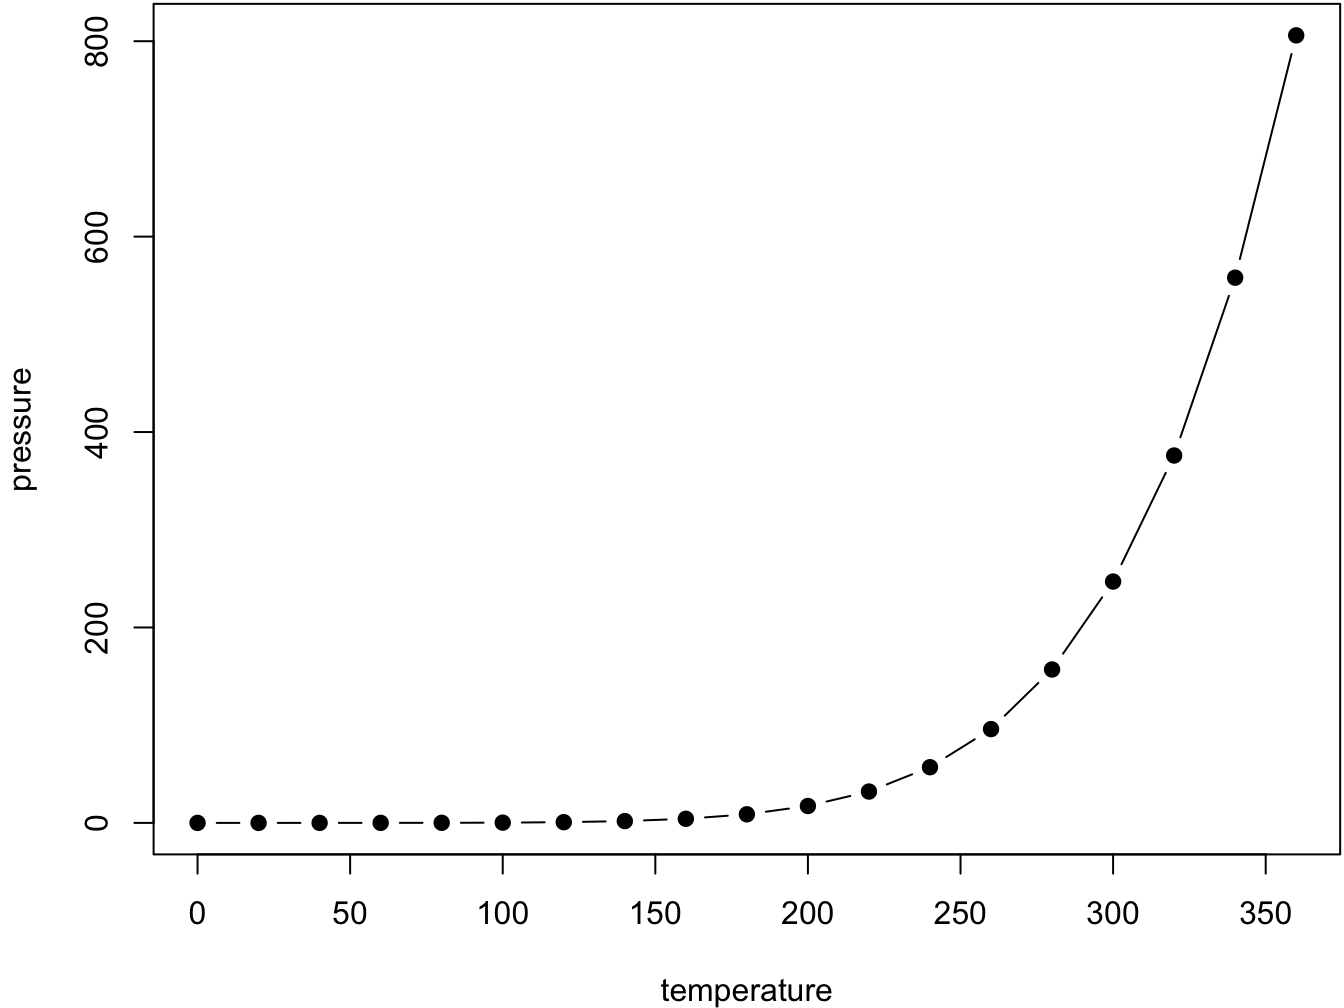
\includegraphics[width=0.8\linewidth]{bookdown-demo_files/figure-latex/nice-fig-1} 

}

\caption{Here is a nice figure!}\label{fig:nice-fig}
\end{figure}

Reference a figure by its code chunk label with the \texttt{fig:} prefix, e.g., see Figure \ref{fig:nice-fig}. Similarly, you can reference tables generated from \texttt{knitr::kable()}, e.g., see Table \ref{tab:nice-tab}.

\begin{Shaded}
\begin{Highlighting}[]
\NormalTok{knitr}\OperatorTok{::}\KeywordTok{kable}\NormalTok{(}
  \KeywordTok{head}\NormalTok{(iris, }\DecValTok{20}\NormalTok{), }\DataTypeTok{caption =} \StringTok{'Here is a nice table!'}\NormalTok{,}
  \DataTypeTok{booktabs =} \OtherTok{TRUE}
\NormalTok{)}
\end{Highlighting}
\end{Shaded}

\begin{table}[t]

\caption{\label{tab:nice-tab}Here is a nice table!}
\centering
\begin{tabular}{rrrrl}
\toprule
Sepal.Length & Sepal.Width & Petal.Length & Petal.Width & Species\\
\midrule
5.1 & 3.5 & 1.4 & 0.2 & setosa\\
4.9 & 3.0 & 1.4 & 0.2 & setosa\\
4.7 & 3.2 & 1.3 & 0.2 & setosa\\
4.6 & 3.1 & 1.5 & 0.2 & setosa\\
5.0 & 3.6 & 1.4 & 0.2 & setosa\\
\addlinespace
5.4 & 3.9 & 1.7 & 0.4 & setosa\\
4.6 & 3.4 & 1.4 & 0.3 & setosa\\
5.0 & 3.4 & 1.5 & 0.2 & setosa\\
4.4 & 2.9 & 1.4 & 0.2 & setosa\\
4.9 & 3.1 & 1.5 & 0.1 & setosa\\
\addlinespace
5.4 & 3.7 & 1.5 & 0.2 & setosa\\
4.8 & 3.4 & 1.6 & 0.2 & setosa\\
4.8 & 3.0 & 1.4 & 0.1 & setosa\\
4.3 & 3.0 & 1.1 & 0.1 & setosa\\
5.8 & 4.0 & 1.2 & 0.2 & setosa\\
\addlinespace
5.7 & 4.4 & 1.5 & 0.4 & setosa\\
5.4 & 3.9 & 1.3 & 0.4 & setosa\\
5.1 & 3.5 & 1.4 & 0.3 & setosa\\
5.7 & 3.8 & 1.7 & 0.3 & setosa\\
5.1 & 3.8 & 1.5 & 0.3 & setosa\\
\bottomrule
\end{tabular}
\end{table}

You can write citations, too. For example, we are using the \textbf{bookdown} package \citep{R-bookdown} in this sample book, which was built on top of R Markdown and \textbf{knitr} \citep{xie2015}.

\hypertarget{literature}{%
\chapter{Literature}\label{literature}}

Here is a review of existing methods.

\hypertarget{methods}{%
\chapter{Methods}\label{methods}}

We describe our methods in this chapter.

\hypertarget{applications}{%
\chapter{Applications}\label{applications}}

Some \emph{significant} applications are demonstrated in this chapter.

\hypertarget{example-one}{%
\section{Example one}\label{example-one}}

\hypertarget{example-two}{%
\section{Example two}\label{example-two}}

\hypertarget{final-words}{%
\chapter{Final Words}\label{final-words}}

We have finished a nice book.

\hypertarget{external}{%
\chapter{External server}\label{external}}

\hypertarget{about-bplim}{%
\section{\texorpdfstring{{About BPLIM}}{About BPLIM}}\label{about-bplim}}

The ability to collect and accumulate microdata has been a powerful
function of central banks. In the scientific community, an increasing
number of research has been conducted using the micro-level
information. To enhance collaborations between the central bank and
the researchers, an advanced data sharing platform is essential.
Accordingly, the Banco de Portugal Microdata Research Laboratory
(BPLIM) (\emph{Laboratório de Investigação em Microdados do Banco de
Portugal}) is created to facilitate future scientific research effort
that incorporates the use of microdata. By eliminating the data access
barrier, BPLIM aims to inspire researches that effectively utilize the
Portuguese administrative micro datasets and contribute to our
understanding of the economic and financial challenges of our time.

\hypertarget{data-confidentiality}{%
\section{\texorpdfstring{{Data Confidentiality}}{Data Confidentiality}}\label{data-confidentiality}}

While researchers prefer unrestricted access to data, care must be
given to secure the confidentiality of the data providers. All access
granted to microdata should obey the applicable law and the data
should only be used for research purposes.

Therefore, the data is only made available to the Banco de Portugal's
internal researchers and those approved external researchers who have
agreed to the bank's legal provisions concerning the use of its data.
Specifically, each external researcher is required to sign a
Confidentiality Agreement with the bank and will only be allowed to
access a customized set of data that is tailored to his/her research
needs. All micro data sets made accessible to external researchers
will be anonymized and stored in information systems belonging to
Banco de Portugal (BdP).

Type of access to the Microdata varies according to levels of
confidentiality (low, medium, high).

\begin{itemize}
\item
  \textbf{Low}: information that can be obtained to the public or
  scientific community by other institutions
\item
  \textbf{Medium}: information pertaining to institutions (firms, banks,
  etc.) not included in the previous case (some CB, CRC Firms, Bank
  Balance Sheet Data).
\item
  \textbf{High}: information about individuals or households not included
  in the \textbf{Low} case (CRC Individuals).
\end{itemize}

\hypertarget{access-to-the-external-server}{%
\section{\texorpdfstring{{Access to the External Server}}{Access to the External Server}}\label{access-to-the-external-server}}

\begin{enumerate}
\def\labelenumi{\arabic{enumi}.}
\tightlist
\item
  Upon access approval, the User will be able to connect to the external server using one of two possibilities.
\end{enumerate}

\begin{itemize}
\tightlist
\item
  NoMachine client access ({preferred}): see \textbf{Appendix 4} for details on installation and use
\item
  Browser access ({low performance}): see \textbf{Appendix 5} for further details
\end{itemize}

\begin{enumerate}
\def\labelenumi{\arabic{enumi}.}
\setcounter{enumi}{1}
\tightlist
\item
  Password policy:
\end{enumerate}

\begin{itemize}
\tightlist
\item
  The first password delivered must be changed at the first login.
\item
  After 60 days the password will expire: change the password within this time frame (see Appendix 3 for instructions on how to change the password)
\item
  The passwords to be specified must meet the requirements described in Appendix 3.
\end{itemize}

\begin{enumerate}
\def\labelenumi{\arabic{enumi}.}
\setcounter{enumi}{2}
\tightlist
\item
  Upon access using `NoMachine'
\end{enumerate}

These are the first three screens you will see

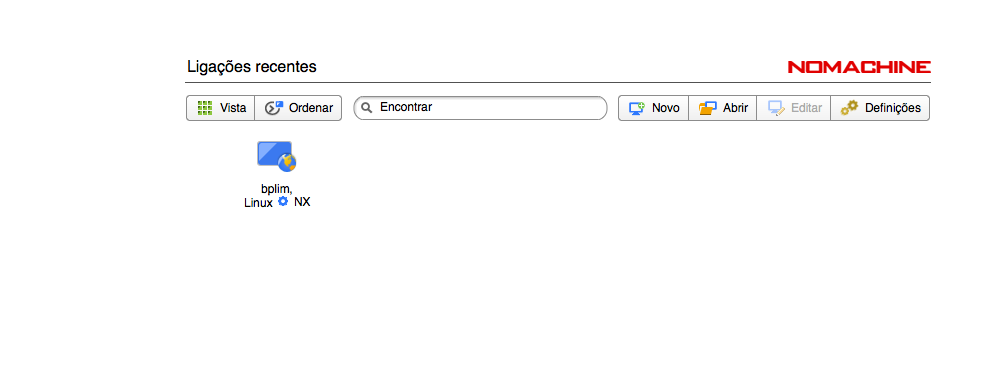
\includegraphics[width=4.72441in,height=1.72233in]{./media/image1.png}

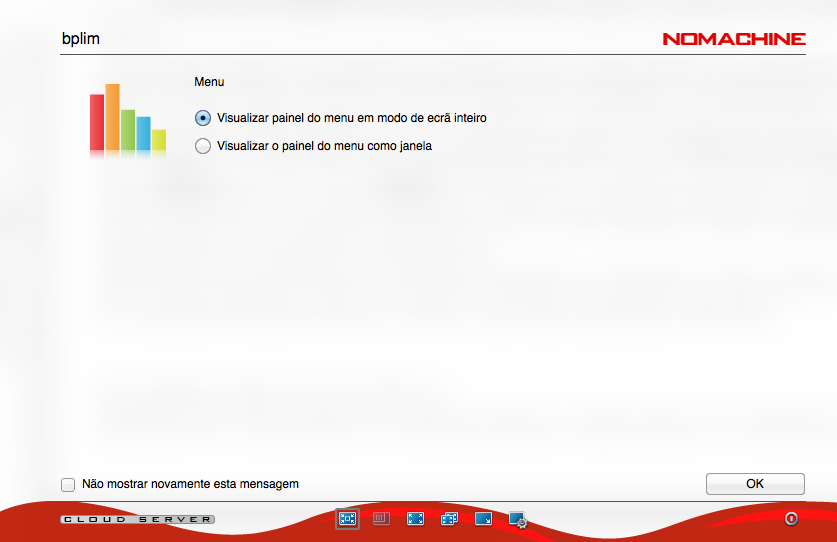
\includegraphics[width=4.72441in,height=3.05928in]{./media/image2.png}

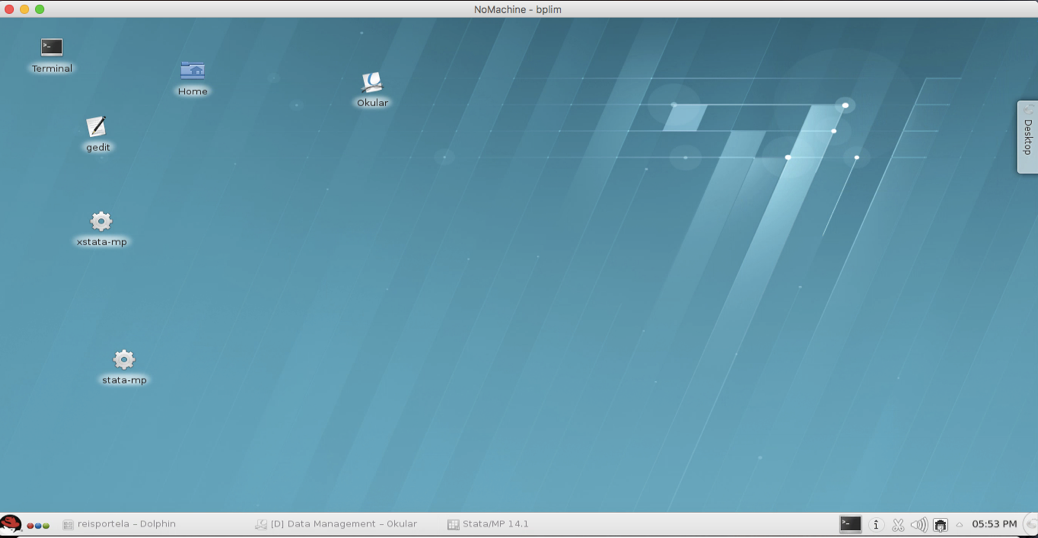
\includegraphics[width=4.72441in,height=2.44898in]{./media/image3.png}

\begin{enumerate}
\def\labelenumi{\arabic{enumi}.}
\setcounter{enumi}{3}
\tightlist
\item
  Select the ``\textbf{Kickoff Application Launcher}'' menu (in the lower left corner):
\end{enumerate}


\includegraphics[width=0.57067in,height=0.56371in]{./media/image4.png}

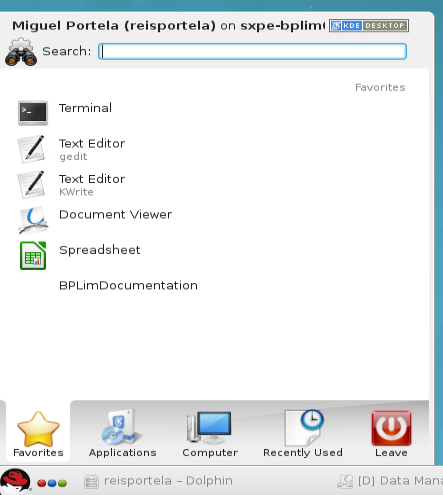
\includegraphics[width=2.3622in,height=2.63948in]{./media/image5.png}

\begin{enumerate}
\def\labelenumi{\arabic{enumi}.}
\setcounter{enumi}{4}
\tightlist
\item
  Then you should:
\end{enumerate}

\begin{itemize}
\tightlist
\item
  Click on the ``\textbf{Applications}'' button
\item
  Select \textbf{``BPLIM''} and click on your project (i.e., ``pxxx\_name''). At this stage, you should see a graphical environment (`Dolphin' application\footnote{Dolphin is an intuitive and easy-to-use file manager. You can use it, for example, to browse the directory, to
    create or to delete files/directories (by using the right mouse
    button). For more information about Dolphin, please visit:
    \href{https://translate.google.com/translate?hl=en\&prev=_t\&sl=pt-BR\&tl=en\&u=https://userbase.kde.org/Dolphin}{\emph{{https://userbase.kde.org/Dolphin}}}
    .}) like this:
\end{itemize}

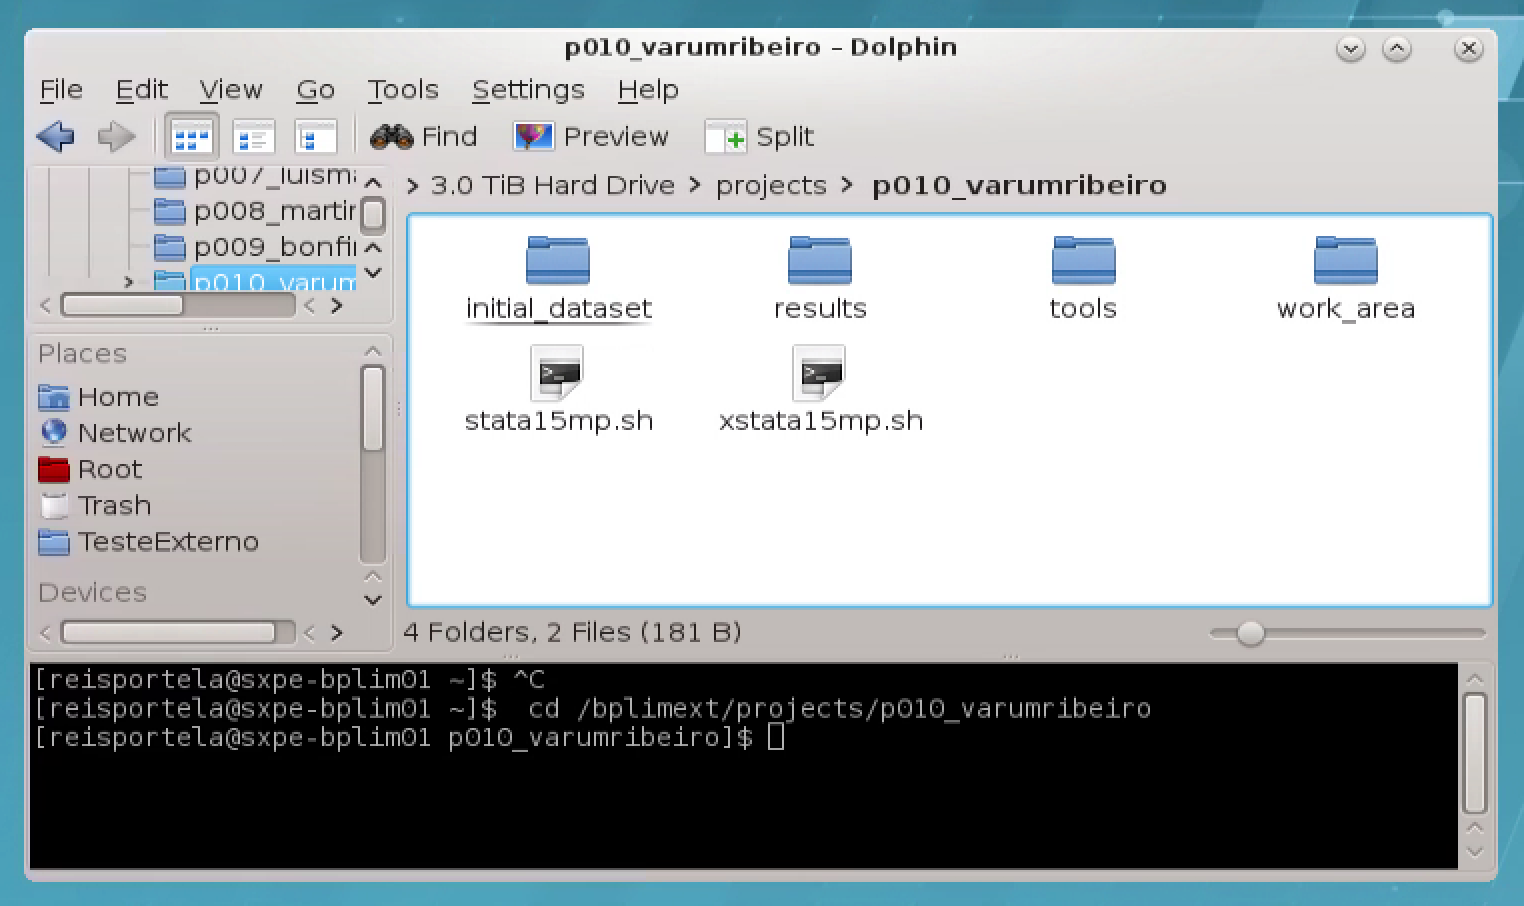
\includegraphics[width=4.72441in,height=2.80866in]{./media/image6.png}

You can see the prompt command line together with `Dolphin' using the
keyboard shortcut `F4'.

The directories that you have access to within the folder include:

\begin{longtable}[]{@{}ll@{}}
\toprule
\endhead
\begin{minipage}[t]{0.47\columnwidth}\raggedright
\textbf{initial\_dataset}\strut
\end{minipage} & \begin{minipage}[t]{0.47\columnwidth}\raggedright
Data sources provided by BPLIM.

\emph{You have
read-only access to this
directory.}\strut
\end{minipage}\tabularnewline
\begin{minipage}[t]{0.47\columnwidth}\raggedright
\textbf{results}\strut
\end{minipage} & \begin{minipage}[t]{0.47\columnwidth}\raggedright
Output files that
researchers wish to generate
and extract from the server.

\emph{You
have read-write access to this
directory.}\strut
\end{minipage}\tabularnewline
\begin{minipage}[t]{0.47\columnwidth}\raggedright
\textbf{tools}\strut
\end{minipage} & \begin{minipage}[t]{0.47\columnwidth}\raggedright
Specific analysis tools.

\emph{You have read-only access to
this directory.}\strut
\end{minipage}\tabularnewline
\begin{minipage}[t]{0.47\columnwidth}\raggedright
\textbf{work\_area}\strut
\end{minipage} & \begin{minipage}[t]{0.47\columnwidth}\raggedright
Temporary
work directory.

\emph{You have read-write
access to this directory.}\strut
\end{minipage}\tabularnewline
\bottomrule
\end{longtable}

\begin{itemize}
\item
  By default you also have two files (see image above): (1)
  stata15mp.sh; (2) xstata15mp.sh. Files with the
  "\textbf{{sh}}" extension allow you to send commands to
  your operating system or to enter your operating system for
  interactive use. The first one starts Stata version 15 in
  non-graphical mode, while the second launches Stata 15 in
  graphical mode. You can start both applications by typing in the
  Linux shell, for example, `xstata15mp.sh', or by double clicking
  the file name in `Dolphin'\footnote{In case `xstata15mp.sh' does not launch Stata please see `Section
    5.1.b'.}
\item
  To reset and disconnect the remote desktop connection or session,
  you can simply log out your remote session, as shown on the
  screenshot below. After you log out, close the window.\footnote{Click on the cross button at the upper right corner to close.}
\end{itemize}

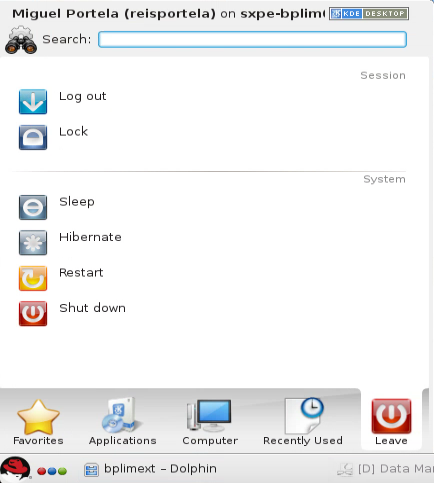
\includegraphics[width=3.14961in,height=3.50521in]{./media/image7.png}

Confirm before exiting by clicking on the \textbf{"Logout"} button to close the window\footnote{Note that before exiting the server, you need to make
  sure that all active programs have been closed (unless they have
  been launched in \emph{batch} mode). Running programs in \emph{batch} mode is justified for
  procedures that require high computational resources, intense
  calculation and / or long processing time.}

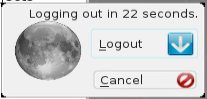
\includegraphics[width=1.14236in,height=0.52288in]{./media/image8.png}

\begin{itemize}
\tightlist
\item
  In case you do not logout, your session will be left open until your
  next login. You may use this facility to run your programs. However,
  one must be aware that this option uses resources from the server,
  so the efficient solution to run your programs ``over night'' is using
  the batch mode as described in Step 6 below. Furthermore, in case
  the server is rebooted during a maintenance procedure your session
  will be automatically close and unsaved documents will be lost. We
  recommend you save at regular intervals your statistical programs.
\end{itemize}

\hypertarget{using-the-shell-in-a-linux-operating-system}{%
\section{\texorpdfstring{{Using the `shell' in a Linux Operating System}}{Using the `shell' in a Linux Operating System}}\label{using-the-shell-in-a-linux-operating-system}}

If you wish to run your
programs in \textbf{\emph{{batch}}} mode, then you must use the
\emph{`\textbf{shell}'} of Linux. You can also use the `shell' to organize the
files in your working space.

\begin{enumerate}
\def\labelenumi{\arabic{enumi}.}
\tightlist
\item
  The \emph{`\textbf{shell}'}\footnote{The '\emph{shell'} supports the commands in Linux operating system
    (some are disabled).}
  {[}\^{}{[}5{]}\{.underline\}\^{}{]}(\url{https://translate.googleusercontent.com/\#footnote5})
  do Linux pode ser aberta a partir d e in Linux can be accessed from
\end{enumerate}

RedHat \textgreater{} ApplicationsApplications \textgreater{}\textgreater{} SystemSystem\textgreater{} \textgreater{}Terminal
Terminal

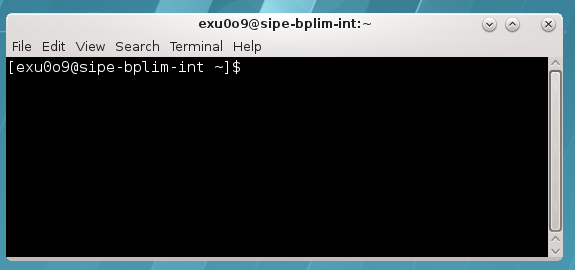
\includegraphics[width=3.93701in,height=1.84868in]{./media/image9.png}

\begin{enumerate}
\def\labelenumi{\arabic{enumi}.}
\setcounter{enumi}{1}
\item
  See the Appendix for a list of some of the most used commands.
\item
  In case you are using a non-English keyboard, the `true' keyboard
  might be different from the one you see. The changes apply mostly
  to the symbols, not letters or numbers. For example, in case you
  have a Portuguese keyboard on your computer the `+' is now in key
  `?', or the `*' is in SHIFT + ?. This issue is specific to the
  Operating System of your computer
\item
  Remember that Linux is case-sensitive: e.g., ``LS'' and ``ls'' are
  treated as different commands.
\item
  You can use the arrow keys to scroll up and down through the
  commands you've entered.
\item
  You can use the ``Tab'' key to complete the command line
  automatically.
\item
  E.g., type the following line to list elements within a folder in a
  `human readable' format, h, long list format, l, in reverse order,
  r, sort by modification time, t, and almost all files, A,

  ls -lArth
\end{enumerate}

\hypertarget{using-stata}{%
\section{\texorpdfstring{{Using Stata}}{Using Stata}}\label{using-stata}}

\begin{enumerate}
\def\labelenumi{\arabic{enumi}.}
\tightlist
\item
  Stata can be accessed in interactive graphical or non-graphical
  modes.\footnote{The version of Stata on the server has the same features as the
    Stata on Windows or Mac. By default when the Stata starts in this
    way the "working directory" active becomes your folder
    "work\_area".}
\end{enumerate}

\begin{itemize}
\item
  Interactive non-graphical mode

  Move to the desired folder, e.g.,

  cd /bplimext/projects/I001\_jdoe/

  and type

  /opt/bplimext/stata15/stata-mp
\end{itemize}

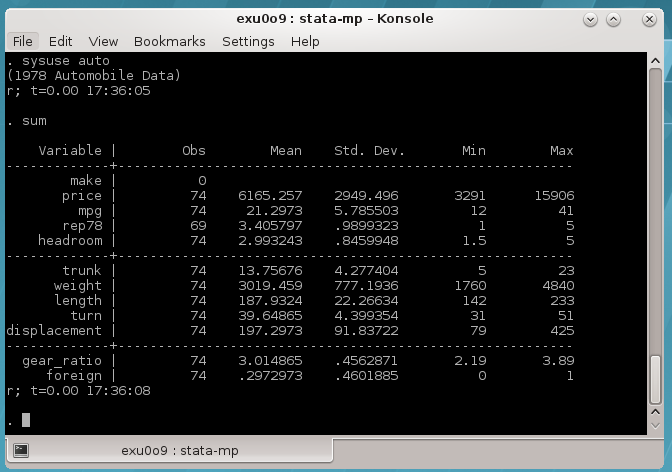
\includegraphics[width=3.54331in,height=2.4886in]{./media/image10.png}

\begin{itemize}
\item
  You may add a `path' to your system folder by typing, for the
  example on Stata 15, the following command in the shell

  PATH = \$PATH:/opt/bplimext/stata15
\item
  For the interactive graphical mode click on the icons
  ``\textbf{{xstata14mp.sh}}'' (Stata 14) or
  ``\textbf{{xstata15mp.sh}}'' (Stata 15) located in the
  `desktop', depending on the desired Stata version,
\end{itemize}

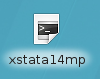
\includegraphics[width=0.59055in,height=0.46654in]{./media/image11.png}

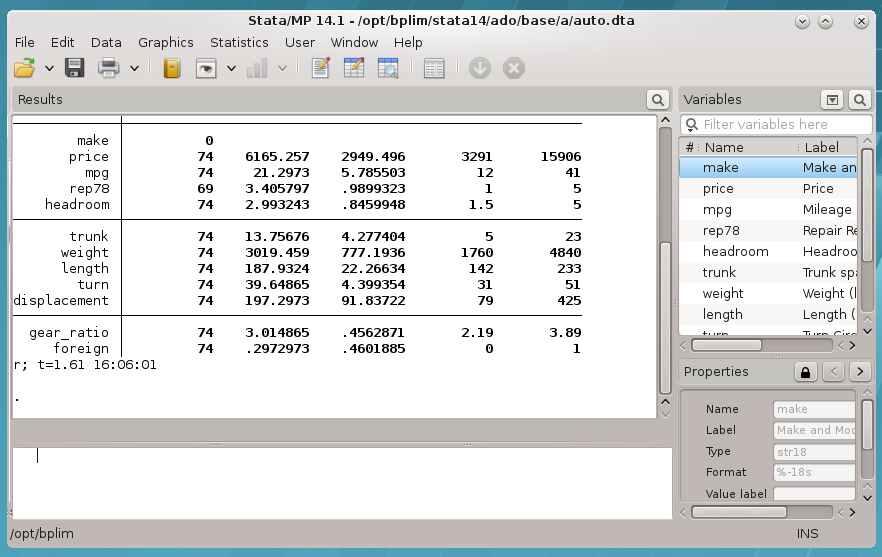
\includegraphics[width=3.93701in,height=2.48638in]{./media/image12.png}

\begin{verbatim}
- You can use the 'Do-file Editor' in Stata to create your own
  "do-files" and "ado-files", or alternatively you can use
  **KWrite** editor (or 'gedit'). Poder á abri-lo a partir de
  **[RedHat]{.underline}** \>

- You can open it from **RedHat** \> **Applications**
  **Applications** \>\> **Utilities** **Utilities** \> \> **KWrite**
  . **KWrite**. You can also launch 'KWrite' from the 'shell' by
  typing 'kwrite'
\end{verbatim}

\begin{itemize}
\tightlist
\item
  In case the icon is not in your desktop, use Dolphin, move to folder
  `/opt/bplimext/stata15', and drag and drop the file `xstata-mp' into
  the desktop
\end{itemize}

\begin{enumerate}
\def\labelenumi{\arabic{enumi}.}
\setcounter{enumi}{1}
\tightlist
\item
  To look for \textbf{``ado-files''}:
\end{enumerate}

``Ado-files'' are text files containing the Stata program. It is
advisable that one create and save his/her ``ado-files'' so the results
can be replicated later by running the saved ``ado-files'' on the
BPLIM's datasets.

Stata looks for ``ado-files'' in several places. When it comes to
personal ado-directories, they can be categorized in four ways:

\begin{itemize}
\item
  (SITE), the directory for ``ado-files'' your site might have
  installed;
\item
  (PLUS), the directory for ``ado-files'' you personally might have
  installed;
\item
  (PERSONAL), the directory for ``ado-files'' you might have written;
\item
  (OLDPLACE), the directory where Stata users used to save their
  personally written ado-files.
\end{itemize}

The ado-files you have just written or those created for this project
can be found in the current directory (.).

Specific `ado-files' you may ask to be made available in the server
will be placed in your folder
`/bplimext/projects/YOURPROJECTID/tools'. You should add this folder
to your Stata `ado-files' folder by executing the following command
within Stata,

sysdir set PERSONAL ``/bplimext/projects/YOURPROJECTID/tools''

You may also edit your `profile.do' file, located in your root folder,
``/home/YOURPROJECTID/'', and add key instructions you may want to be
executed every time you start Stata. The above instruction is one of
such cases. You can create, or edit, the file `profile.do' using
`Do-file Editor' within Stata (`vi profile.do' or KWrite are also a
possibility).

The \textbf{\emph{sysdir}} command within Stata will tell you where they are on
your computer:

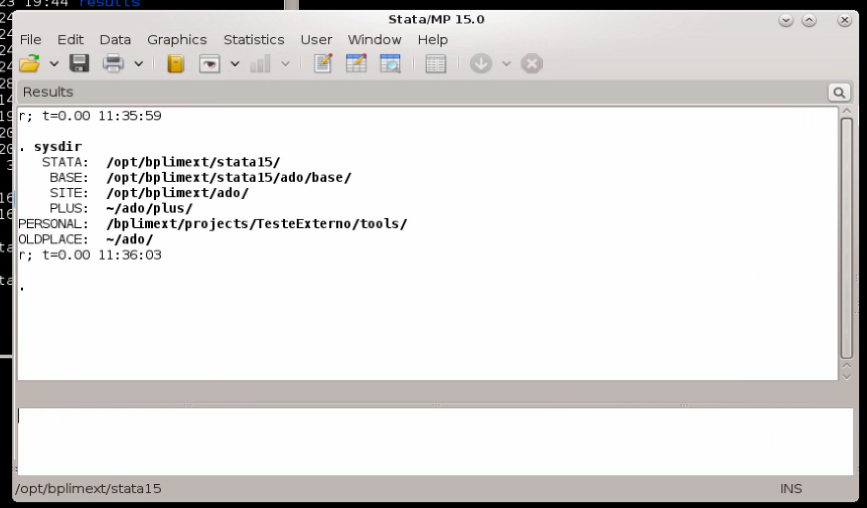
\includegraphics[width=3.93681in,height=2.27514in]{./media/image13.png}

\hypertarget{stata-in-batch-mode}{%
\section{\texorpdfstring{{Stata in `batch' mode}}{Stata in `batch' mode}}\label{stata-in-batch-mode}}

\begin{enumerate}
\def\labelenumi{\arabic{enumi}.}
\tightlist
\item
  Start a \emph{'\textbf{shell}'} in Linux and navigate to the directory
  of the ``do-file'' file that you want to run (ex: prog1.do)
\end{enumerate}

\textbf{cd /bplim/projects/I001\_jdoe/work\_area/} cd
/bplimext/projects/I001\_jdoe/work\_area/

\begin{enumerate}
\def\labelenumi{\arabic{enumi}.}
\setcounter{enumi}{1}
\tightlist
\item
  You might find it easier to use `Dolphin' (= File Manager) to move
  over your folder structure. In this case, we recommend activating
  the `shell' (= `Terminal') associated with `Dolphin'
\end{enumerate}

\begin{itemize}
\item
  use Dolphin/File Manager
\item
  click `F4' to activate the shell with Dolphin. Benefit: fast
  transition within folders and, at the same time, the ability
  to run shell commands
\end{itemize}

\begin{enumerate}
\def\labelenumi{\arabic{enumi}.}
\setcounter{enumi}{2}
\item
  Create an ASCII file named, e.g., `batch\_prog1'
\item
  Inside the file write just a line with the execution command you
  would type in the `shell'; e.g.,

  /opt/bplimext/stata15/stata-mp do
  /bplimext/projects/BPlim\_inicial/work\_area/prog1.do
\item
  You can use, for example, the command line app `vi' to create the batch file
\end{enumerate}

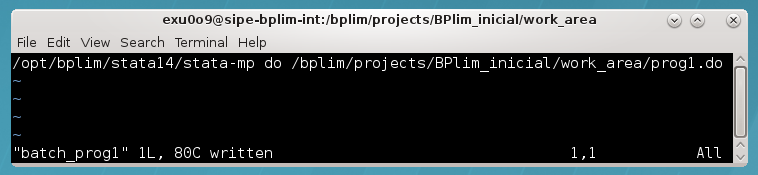
\includegraphics[width=3.54331in,height=0.81802in]{./media/image14.png}

\begin{enumerate}
\def\labelenumi{\arabic{enumi}.}
\setcounter{enumi}{5}
\tightlist
\item
  The batch file can also be created using apps like `kwrite' or Stata
  `do file editor'
\end{enumerate}

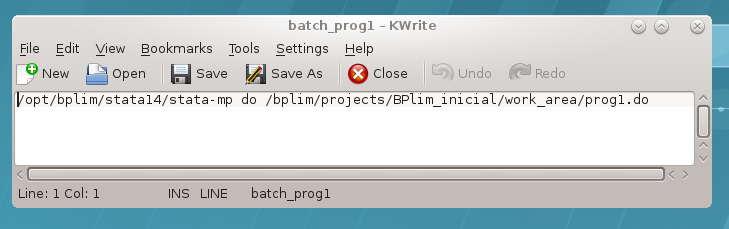
\includegraphics[width=3.54331in,height=1.11324in]{./media/image15.png}

or

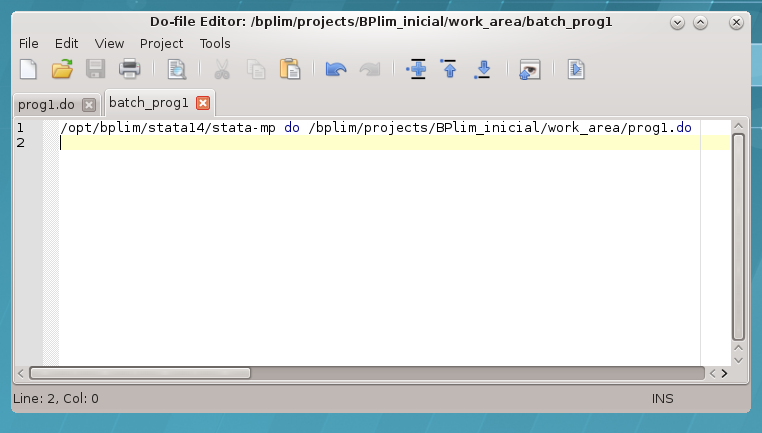
\includegraphics[width=3.54331in,height=2.01342in]{./media/image16.png}

\begin{enumerate}
\def\labelenumi{\arabic{enumi}.}
\setcounter{enumi}{6}
\item
  You may add the extension `.txt' to the name of the batch file, as
  sometimes Stata \emph{doeditor} does not `see' the file `batch', while
  it `sees' `batch.txt'
\item
  Once the batch file is created one runs the .do file in batch mode
  by typing in the `Terminal':

  at now --f batch.txt
\item
  Type `man at' to see further option of the command `at'; e.g., one
  could type

  at now + 5 hours --f batch.txt
\end{enumerate}

or

\begin{verbatim}
at now + 4 minutes --f batch\_prog1
\end{verbatim}

to run the Stata program within 5 hours or 4 minutes from now,
respectively. `man' is the help function in Linux

\begin{enumerate}
\def\labelenumi{\arabic{enumi}.}
\setcounter{enumi}{9}
\item
  Type `top' in the shell/Terminal to confirm the program is running
\item
  Under `top' type `i' to hide irrelevant processes (show less output)
\item
  To kill a running process with `top' press `k', for `kill', write
  \textgreater{} the process number and then type `9'. The process number is
  \textgreater{} identified in the first column as PID
\item
  To get out of the top, type `q'
\item
  Useful features of the command `at':
\end{enumerate}

\begin{itemize}
\item
  `atq': use it to see programs in the batch queue (an `=' sign
  indicates the program is running; an `a' indicates it is in
  the queue and we see the time when it will be executed)
\item
  `atrm \#': remove a batch from the batch queue
\item
  one can see how the batch is running by typing

  `tail --f logcrc\_may21.log'
\end{itemize}

It allows you to see an updated version of the last lines of the log;
\emph{i.e.}, it updates each time the log is changed by Stata. A key
advantage of tail is that it does not interfere with the log file,
namely it does not write over it.

\begin{enumerate}
\def\labelenumi{\arabic{enumi}.}
\setcounter{enumi}{14}
\tightlist
\item
  Another way to run a program in the background is by using the
  command `screen'
\end{enumerate}

\begin{itemize}
\item
  `screen' is useful when one wants to run Stata in interactive
  mode and still guarantee that if the network connection goes
  down one does not lose the session. We can simply kill the
  `NoMachine' session and recover it later by typing `screen
  --r'
\item
  We can run several instances of screen. If this is the case,
  after opening a new NoMachine session we need to type in the
  Terminal shell `screen --d' to identify the running background
  sessions. We can retrieve a particular session by knowing the
  `pid' number and typing `screen --r 34176'
\end{itemize}

\hypertarget{additional-statistical-software}{%
\section{\texorpdfstring{{Additional Statistical Software}}{Additional Statistical Software}}\label{additional-statistical-software}}

You can also use `R' and `python' by issuing in the shell the
respective designation. Both applications can only be used in the
`shell'. You can check the packages available in R by tipping
`installed.packages()'.

\hypertarget{allowed-outputs}{%
\section{\texorpdfstring{{Allowed outputs}}{Allowed outputs}}\label{allowed-outputs}}

Stata results can be exported to a file on disk using one of the following formats:

\begin{enumerate}
\def\labelenumi{\arabic{enumi}.}
\item
  ASCII files: e.g., log files
\item
  graphs: as .PNG (do not use the option save, or saving, within a
  graph command; instead, use the separate command line `graph export
  xyz.png')
\item
  csv: CSV (Comma Separated Value format), e.g., for use with MS Excel
\item
  rtf: Rich Text Format for use with word processors
\item
  xls or xlsx: Excel files with output tables
\item
  tex: Latex format
\end{enumerate}

\hypertarget{remove-outputs}{%
\section{\texorpdfstring{{Remove outputs}}{Remove outputs}}\label{remove-outputs}}

Place in the ``{results}'' folder all the outputs you want
to remove from the server.\footnote{You may only remove text files that do not contain data or results
  that allow identification. For all the graphs you request as an
  output you must provide the corresponding Table to replicate it. You
  may only export graphs in .PNG format (no vector graph is allowed).}

\begin{enumerate}
\def\labelenumi{\arabic{enumi}.}
\item
  Send an email with the title
  ``\textbf{project I001\_jdoe}: request for result extraction'' to
  ``\textbf{{bplim@bportugal.pt}}''.
\item
  Upon validation, the results will be sent to you via email.
\end{enumerate}

\hypertarget{scientific-support}{%
\section{\texorpdfstring{{Scientific Support}}{Scientific Support}}\label{scientific-support}}

Researchers will be provided with the necessary scientific and
computational support (\emph{i.e.}, advises on programming, computational
resources, micro econometrics, and econometrics of panel data for
research undertaken with the selected Microdata).

\hypertarget{appendix-1-basic-shell-commands-on-linux}{%
\section{\texorpdfstring{{Appendix 1 -- Basic `shell' Commands on Linux}}{Appendix 1 -- Basic `shell' Commands on Linux}}\label{appendix-1-basic-shell-commands-on-linux}}

\begin{itemize}
\item
  \textbf{top} List the procedures that are being executed on the
  server

  \begin{itemize}
  \item
    clicar em ' i ' para omitir processos adormecidos; press 'i'
    \textgreater{} option to omit background processes;
  \item
    clicar press ' h ' para \textbf{\emph{help on top options}} ; 'h'
    \textgreater{} option to obtain the \textbf{top command help}.
  \end{itemize}
\item
  \textbf{pwd} Show current working
  directory
\item
  \textbf{cd} Change directory

  cd /bplimext/projects/I001\_jdoe/work\_area/

  `cd \textasciitilde{}' moves to your home folder
\end{itemize}

\begin{itemize}
\item
  \textbf{cp}cp Copy file(s) to a given path

  cp prog1.do /bplimext/projects/I001\_jdoe/results
\end{itemize}

\begin{itemize}
\item
  \textbf{mv}mv Move file(s) or rename a file from a given path

  mv prog1.do /bplimext/projects/I001\_jdoe/results
\end{itemize}

\begin{itemize}
\item
  \textbf{rm}rm Delete a file

  rm /bplimext/projects/I001\_jdoe/results/prog1.do
\end{itemize}

\begin{itemize}
\item
  \textbf{mkdir}mkdir Creates a directory

  mkdir programas
\end{itemize}

\begin{itemize}
\item
  \textbf{rmdir}rmdir Deletes a directory

  rmdir programas
\end{itemize}

\begin{itemize}
\item
  \textbf{screen}screen Switch between screen

  screen top
\end{itemize}

\begin{itemize}
\item
  \textbf{stata} -- \textbf{mpman}man Show the manual page for the given command

  man ls
\end{itemize}

\begin{itemize}
\tightlist
\item
  \textbf{du}du -h Check the information of disk usage of files and
  directories.
\end{itemize}

\begin{quote}
The ``\textbf{-h}'' option with ``\textbf{du}'' command provides results in ``Human
Readable Format''.
\end{quote}

Ex: du /bplimext/projects/I001\_jdoe/work\_area/

\begin{itemize}
\item
  \textbf{df}df -h Check disk space utilization and show the disk space
  \textgreater{} statistics in ``human readable'' format.
\item
  vi View `ASCII' files; e.g., log files
\item
  \textbf{ghostscript} Preview files with the extensions of \textbf{.eps} and
  \textbf{.pdf}
\end{itemize}

\begin{quote}
ghostscript /bplimext/projects/I001\_jdoe/results/`file\_name.pdf'
\end{quote}

\begin{itemize}
\item
  okular View `PDF'
\item
  find Find files
\end{itemize}

\begin{quote}
Structure: find /path option filename

find . --name ``*.do''

Send the `find' output to a file:

find . --name ``*.do'' \textgreater{} find\_results.txt

Look for a particular string within the `find' output:

find . --name ``*.do'' \textbar{} grep ``analise''

Identify files with extension `.do' that \textbf{contain} the word `graph':

find . --name ``*.do'' -exec grep ``graph export'' `\{\}' \textbackslash{}; -print
\end{quote}

\begin{itemize}
\item
  passwd Change your password
\item
  \textbf{To exit} a program, type \textbf{CTRL + C} (`CTRL + C' kills a particular
  execution in the shell)
\end{itemize}

\hypertarget{appendix-2-using-the-vi-file-editor}{%
\section{\texorpdfstring{{Appendix 2 -- Using the `vi' file editor}}{Appendix 2 -- Using the `vi' file editor}}\label{appendix-2-using-the-vi-file-editor}}

\begin{enumerate}
\def\labelenumi{\arabic{enumi}.}
\item
  In the shell type `vi batch1.txt'
\item
  This are the main shortcut keys

  \begin{enumerate}
  \def\labelenumii{\alph{enumii}.}
  \item
    `i' insert text
  \item
    `ESC' key get out of the `insert' mode
  \item
    `x' delete specific characters
  \item
    `dd' delete a full line
  \item
    `10 dd' delete 10 lines
  \item
    `yy' copy lines
  \item
    `p' paste lines
  \item
    `SHIFT + G' go to the last line
  \item
    `gg' goes to the first line
  \item
    `ESC + q!' exit `vi' without writing
  \item
    `w!' write and replace the file
  \item
    `ESC + q' exit the `vi' session
  \item
    Check, for example,
    \url{https://www.cs.colostate.edu/helpdocs/vi.html}
  \end{enumerate}
\item
  Much easier solution: call `gedit' file editor
\item
  Linux commands I have to add to the manual
\item
  `CTRL + R': allows me to recover a previous command
\item
  vi .bash\_history
\end{enumerate}

\hypertarget{appendix-3-external-servers-password-requirements}{%
\section{\texorpdfstring{{Appendix 3 -- External server's password requirements}}{Appendix 3 -- External server's password requirements}}\label{appendix-3-external-servers-password-requirements}}

\begin{longtable}[]{@{}lll@{}}
\toprule
\endhead
\begin{minipage}[t]{0.30\columnwidth}\raggedright
\textbf{Rule}\strut
\end{minipage} & \begin{minipage}[t]{0.30\columnwidth}\raggedright
\textbf{Value}\strut
\end{minipage} & \begin{minipage}[t]{0.30\columnwidth}\raggedright
\textbf{Notes }\strut
\end{minipage}\tabularnewline
\begin{minipage}[t]{0.30\columnwidth}\raggedright
Maximum Password
Lifetime\strut
\end{minipage} & \begin{minipage}[t]{0.30\columnwidth}\raggedright
\textbf{{60
days}}\strut
\end{minipage} & \begin{minipage}[t]{0.30\columnwidth}\raggedright
\textbf{{After 60 days the
password will
expire}}
and has to be changed
in the next login.
The password can be
changed at any moment
using: \textbf{(1)}, ``All
Applications \textbar{}
Settings \textbar{} System
Settings -- Account
Details'', click
``Change Password'';
or, \textbf{(2)}, in the
`Shell' type `passwd'\strut
\end{minipage}\tabularnewline
\begin{minipage}[t]{0.30\columnwidth}\raggedright
Minimum Number of
Character Classes\strut
\end{minipage} & \begin{minipage}[t]{0.30\columnwidth}\raggedright
4\strut
\end{minipage} & \begin{minipage}[t]{0.30\columnwidth}\raggedright
You should include at
least 4 classes of
characters in the
password. For
example, small
letters, capital
letters, numbers and
punctuation marks.

There are a total of
five classes:

\begin{quote}
1. Capital letters
:
A-Z

2. Small letters:
a-z

3. Numbers: 1-9

4. Punctuation
marks: \textless{}space\textgreater{} !
\% \& ( ) * + . , \{
\} \[ \] \textasciitilde{} " \# \$
' - / \textbackslash{} \^{} \_ `
\textbar{}

5. Characters abov
e
127 (0x7F): marked
characters (ã, á,
ä, à, etc.);
symbols (@, £, §,
º, ª, «, », etc.)
\end{quote}

Number of characters:
by using the same
character 3 or more
times may imply the
use of an additional
class (it is highly
recommended that you
do not use
consecutively the
same character more
than 2 times)\strut
\end{minipage}\tabularnewline
\begin{minipage}[t]{0.30\columnwidth}\raggedright
Minimum Length of
Password\strut
\end{minipage} & \begin{minipage}[t]{0.30\columnwidth}\raggedright
8\strut
\end{minipage} & \begin{minipage}[t]{0.30\columnwidth}\raggedright
The minimum size of
the password is 8
characters (it may be
higher in case you
repeat characters)\strut
\end{minipage}\tabularnewline
\begin{minipage}[t]{0.30\columnwidth}\raggedright
Password History\strut
\end{minipage} & \begin{minipage}[t]{0.30\columnwidth}\raggedright
7\strut
\end{minipage} & \begin{minipage}[t]{0.30\columnwidth}\raggedright
One cannot use a
password defined in
the previous set of 7
passwords\strut
\end{minipage}\tabularnewline
\begin{minipage}[t]{0.30\columnwidth}\raggedright
Maximum Consecutive
Failures\strut
\end{minipage} & \begin{minipage}[t]{0.30\columnwidth}\raggedright
6\strut
\end{minipage} & \begin{minipage}[t]{0.30\columnwidth}\raggedright
If the user fails 6
consecutive times the
password the account
will be locked for
the time defined in
``Lockout Time''\strut
\end{minipage}\tabularnewline
\begin{minipage}[t]{0.30\columnwidth}\raggedright
Fail Interval\strut
\end{minipage} & \begin{minipage}[t]{0.30\columnwidth}\raggedright
60 sec.\strut
\end{minipage} & \begin{minipage}[t]{0.30\columnwidth}\raggedright
Time interval for
attempts to enter a
password to be
considered
consecutive. If more
than 60 seconds have
elapsed since the
last attempt,
consecutive attempts
are no longer
considered, ie the
number of failures,
according to the
requirement "Maximum
Consecutive
Failures" becomes
one.\strut
\end{minipage}\tabularnewline
\begin{minipage}[t]{0.30\columnwidth}\raggedright
Lockout Time\strut
\end{minipage} & \begin{minipage}[t]{0.30\columnwidth}\raggedright
600 sec.\strut
\end{minipage} & \begin{minipage}[t]{0.30\columnwidth}\raggedright
Time (10 minutes)
during which the
account will be
locked if the maximum
number of failed
attempts is reached.\strut
\end{minipage}\tabularnewline
\bottomrule
\end{longtable}

\hypertarget{appendix-4-download-install-and-configure-nomachine-client}{%
\section{\texorpdfstring{{Appendix 4 -- Download, install and configure NoMachine client}}{Appendix 4 -- Download, install and configure NoMachine client}}\label{appendix-4-download-install-and-configure-nomachine-client}}

\textbf{Step 1}: go to the link below and use the credentials provided by
BPLIM to access the site. \textbf{Note}: sometimes the internet provider,
\emph{e.g.}, an University, may block the access to this particular web site.
Please check with your provider in case you get an error while trying to
use the link.

\url{https://www.bportugal.pt/webdrive/index.php/s/irAzxZmir8KHyzD/authenticate}

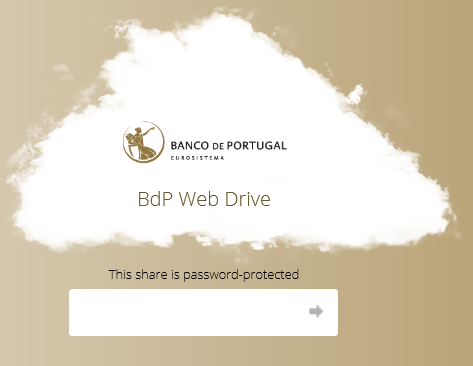
\includegraphics[width=3.0528in,height=2.3622in]{./media/image17.png}

\textbf{Step 2}: download the file with an extension compatible with your OS
(Operation System)

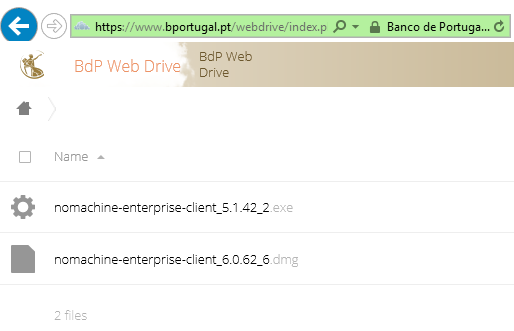
\includegraphics[width=3.6682in,height=2.3622in]{./media/image18.png}

\textbf{Step 3}: install `NoMachine'

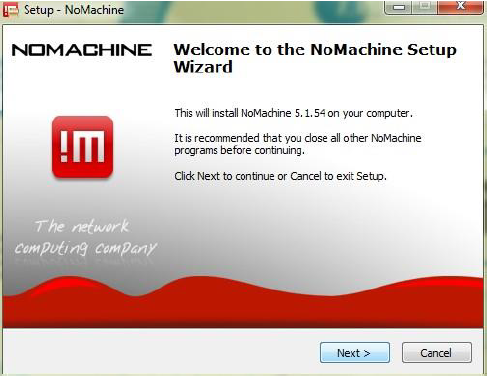
\includegraphics[width=4.07941in,height=3.14961in]{./media/image19.png}

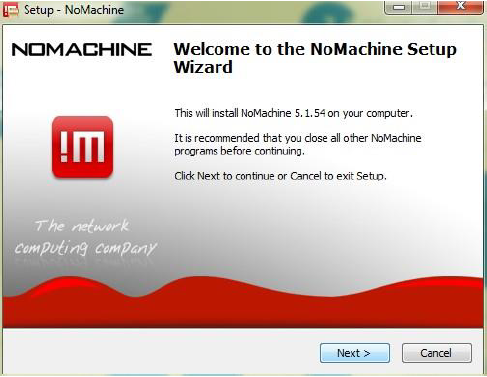
\includegraphics[width=4.06859in,height=3.14961in]{./media/image20.png}

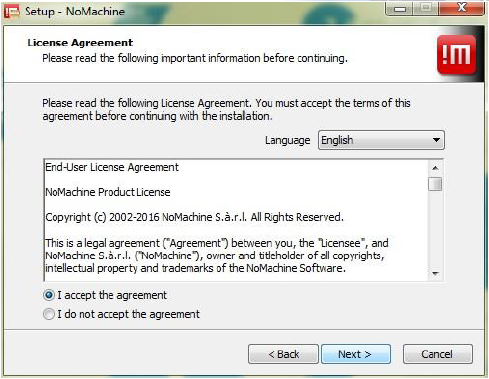
\includegraphics[width=4.06374in,height=3.14961in]{./media/image21.png}

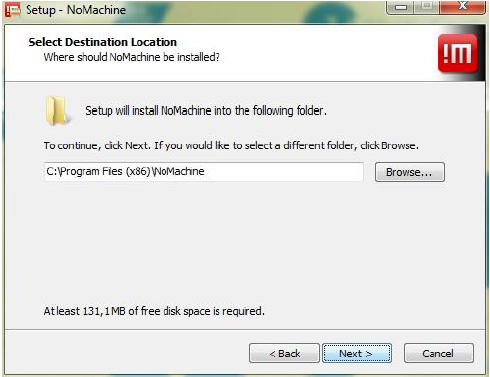
\includegraphics[width=4.09365in,height=3.14961in]{./media/image22.png}

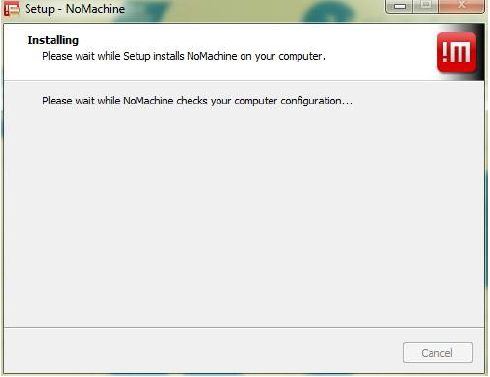
\includegraphics[width=4.09365in,height=3.14961in]{./media/image23.png}

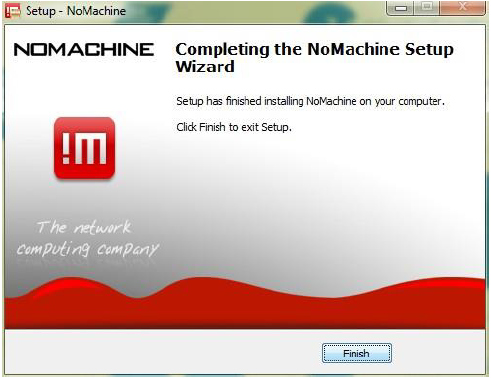
\includegraphics[width=4.09115in,height=3.14961in]{./media/image24.png}

\textbf{\\
}

\textbf{Step 4}: reboot your computer

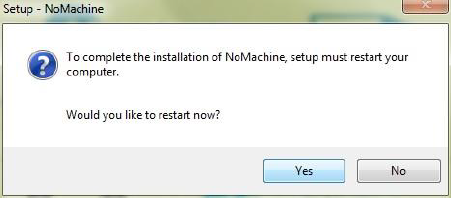
\includegraphics[width=2.75591in,height=1.21602in]{./media/image25.png}

\textbf{Step 5}: NoMachine client access configuration

\textbf{Step 5.1}: start `NoMachine' and create a new connection

\begin{quote}
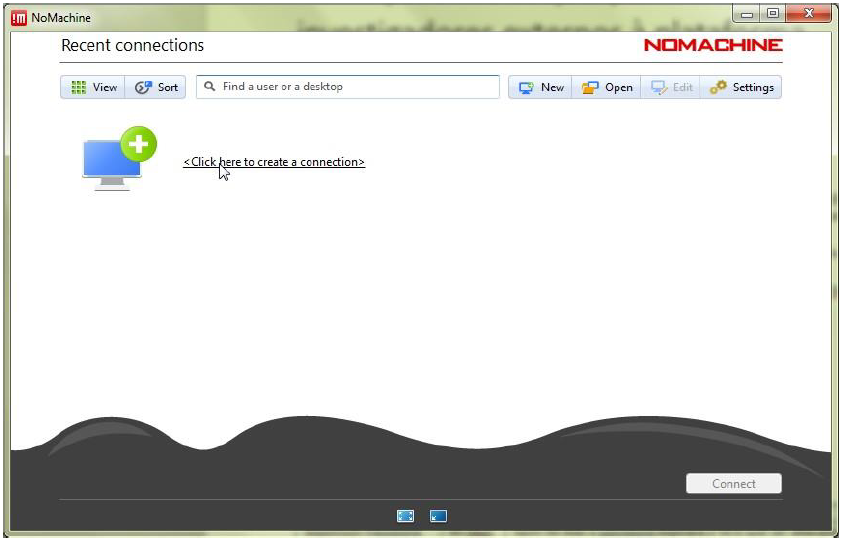
\includegraphics[width=4.72441in,height=3.02971in]{./media/image26.png}
\end{quote}

\textbf{Step 5.2}: Choose `NX protocol'

\begin{quote}
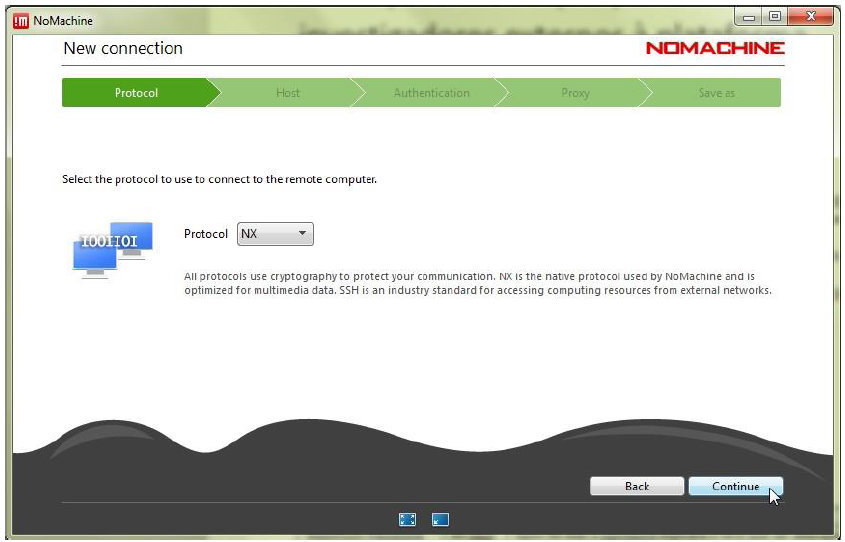
\includegraphics[width=4.72441in,height=3.0302in]{./media/image27.png}
\end{quote}

\textbf{Step 5.3}: Define the `Host' as bplim.bportugal.pt, `Port' 4000

\begin{quote}
Click `Use UDP communication for multimedia data'

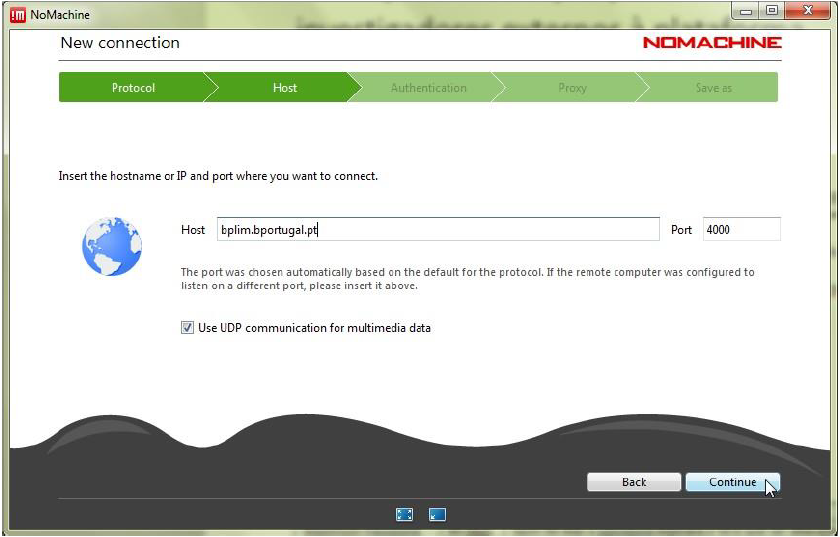
\includegraphics[width=4.72441in,height=3.02002in]{./media/image28.png}

\textbf{Step 5.4}: Use password authentication, with or without proxy,
depending on the instructions of the network administrator / user's
computer support, with the name ``BPLIM-LabInvestMicrodados Banco de
Portugal''.

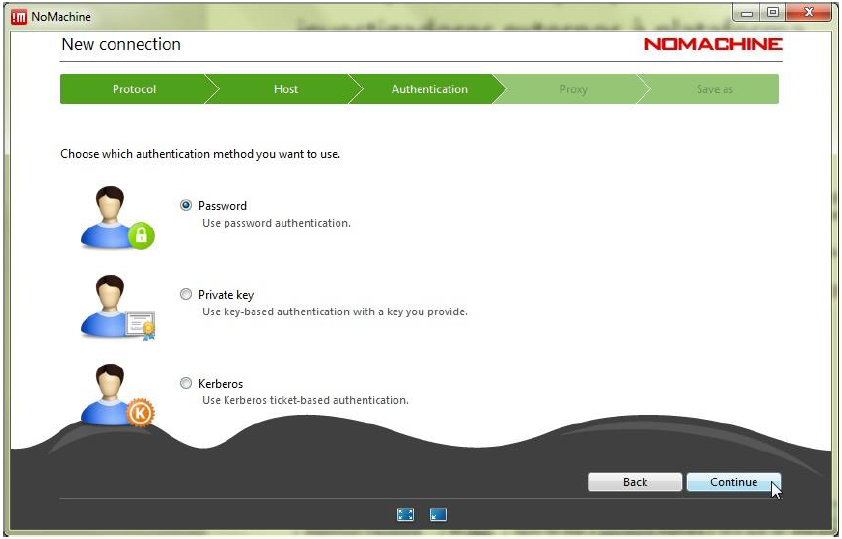
\includegraphics[width=4.72441in,height=3.02438in]{./media/image29.png}

\textbf{Step 5.5}: Do not use a `proxy'

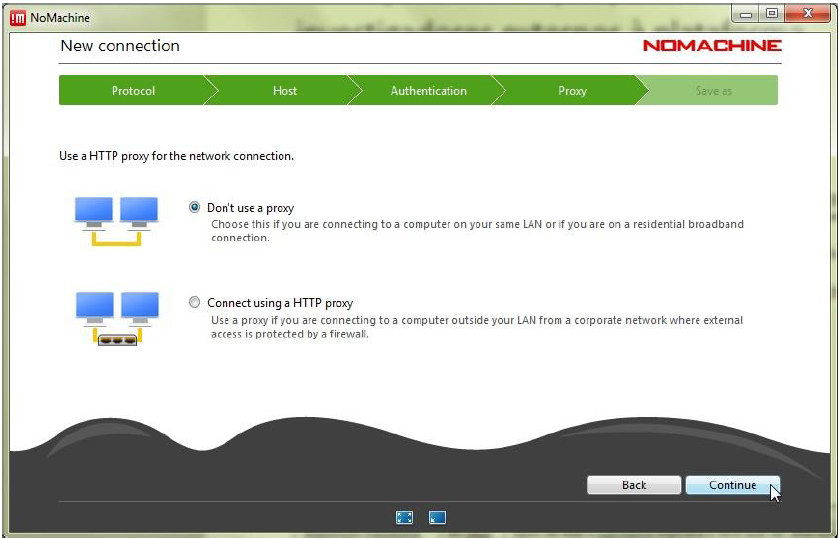
\includegraphics[width=4.72441in,height=3.03165in]{./media/image30.png}

\textbf{Step 5.6}: Define a name for the connection

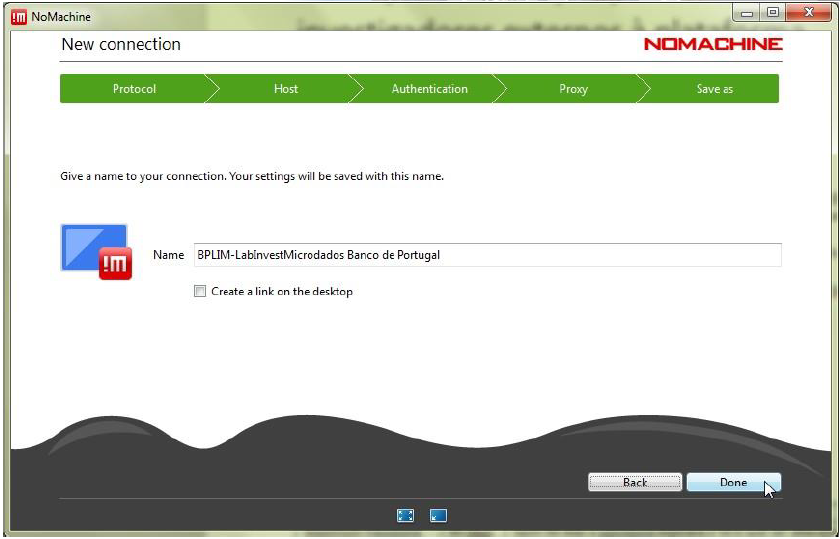
\includegraphics[width=4.72441in,height=3.03165in]{./media/image31.png}

\textbf{Step 5.7}: Once the entry for bplim.bportugal.pt has been created,
connect:

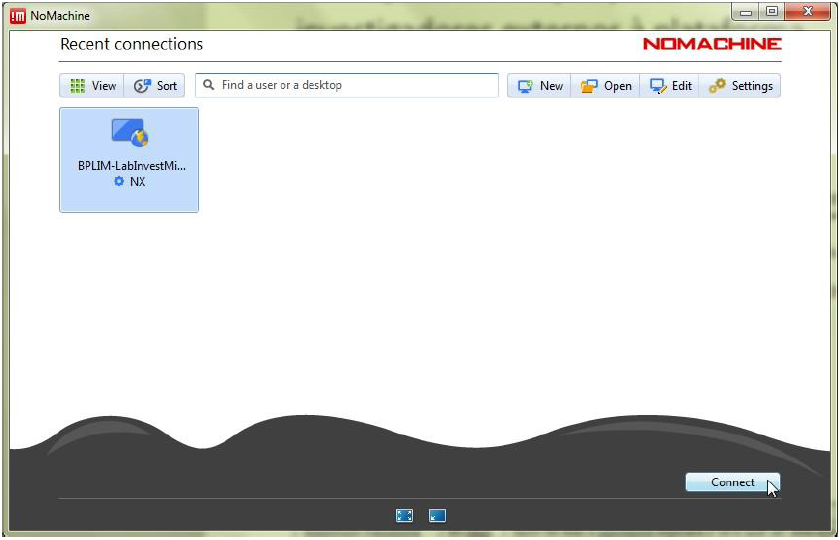
\includegraphics[width=4.72441in,height=3.03698in]{./media/image32.png}
\end{quote}

\textbf{\\
}

\begin{quote}
\textbf{Step 5.8}: Before the first effective connection it may be
necessary to accept the certificate from bplim.bportugal.pt

The Investigator should verify that the "fingerprint" (verification
code) is:

\textbf{29 DC CC 9E 8B 87 23 B1 76 28 8D 29 3F D0 E3 EB 4E 73 76 9D}

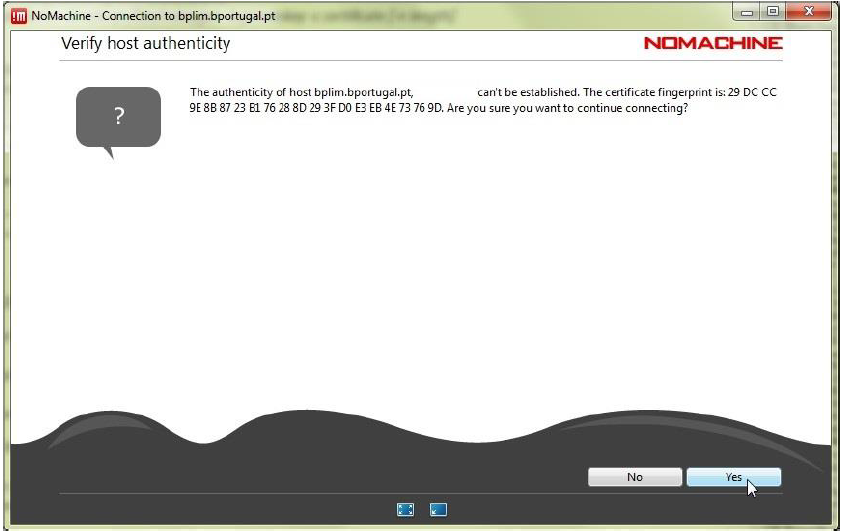
\includegraphics[width=4.72441in,height=2.98511in]{./media/image33.png}
\end{quote}

\textbf{\\
}

\begin{quote}
\textbf{Step 5.9}: Connect with the UserID (\textbf{case sensitive}) and
password provided by Banco de Portugal:

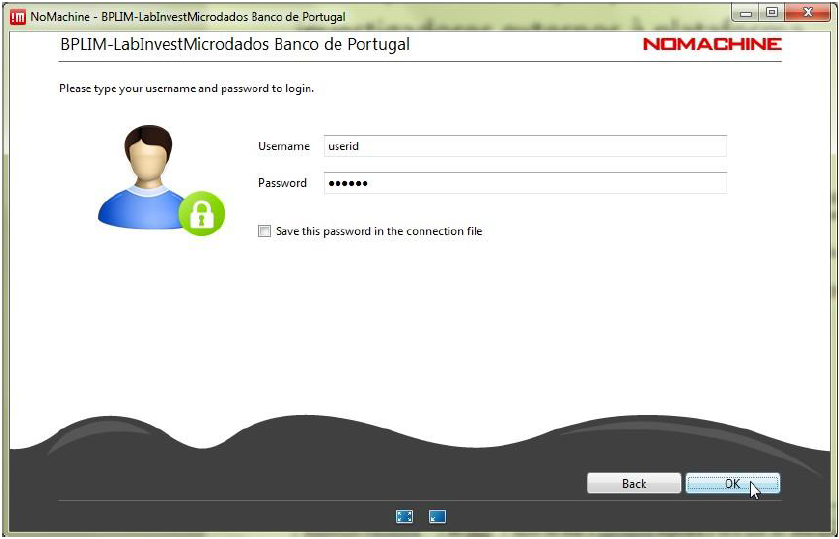
\includegraphics[width=4.72441in,height=3.03504in]{./media/image34.png}

\textbf{Step 5.10}: After the first successful login, it is necessary to
change the password, which must comply with the Password Policy
defined above.

If the new password does not comply with the Password Policy, the
original password provided by the Banco de Portugal will be
re-requested. See Appendix 3 for details.

The NoMachine client does not tell you why the new password was not
accepted -- it is the responsibility of the user to verify that the
new password is in compliance.

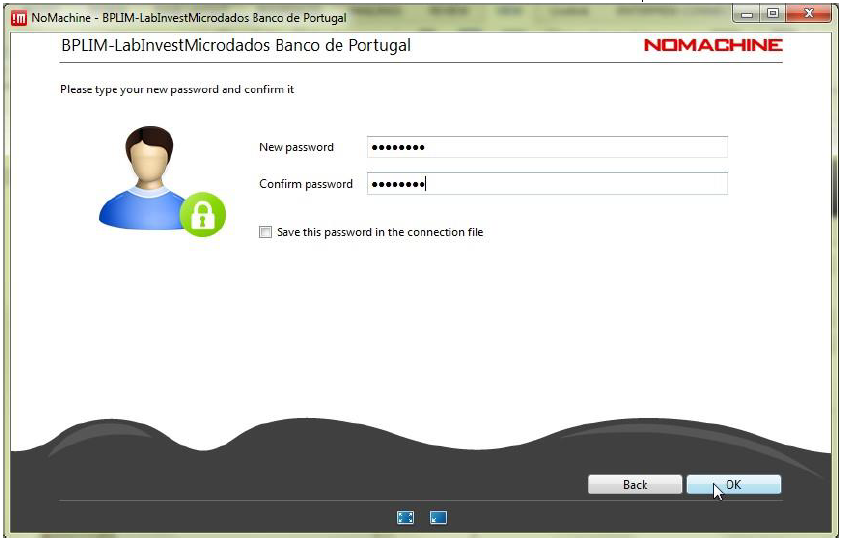
\includegraphics[width=4.72441in,height=3.02972in]{./media/image35.png}

\textbf{Step 5.11}: Upon login success the following screens should appear

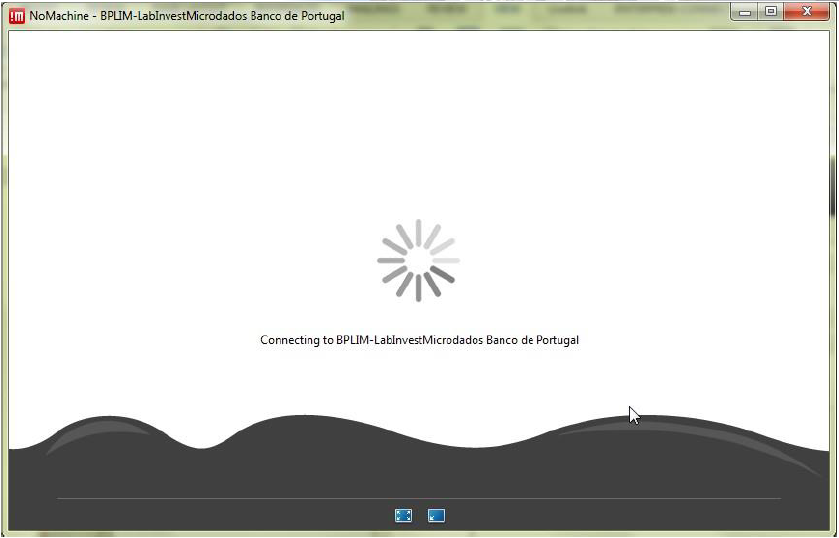
\includegraphics[width=4.72441in,height=3.02971in]{./media/image36.png}

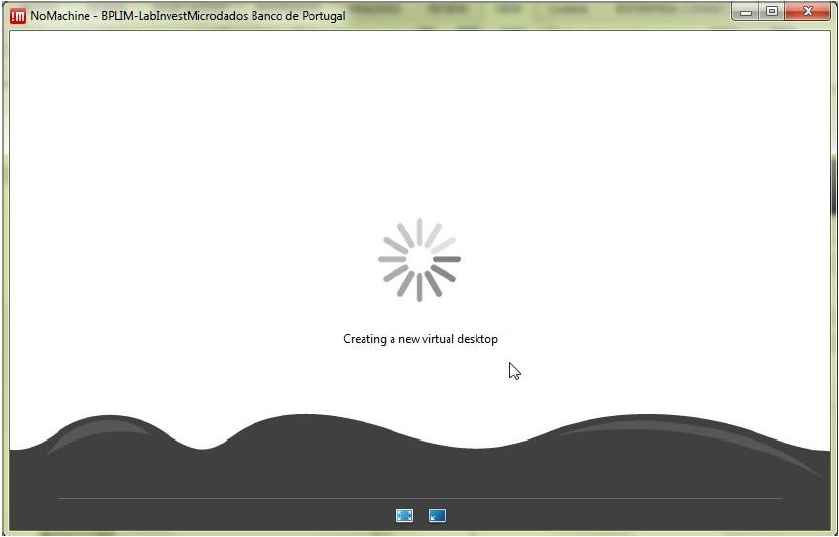
\includegraphics[width=4.72441in,height=3.02389in]{./media/image37.png}

Once logged in and with access to a KDE session, click on the upper
right corner of the KDE desktop, as shown below, to access the menu
and then expand the screen as exemplified for greater ease of use.

\textbf{Step 5.12}: You should see the following screen.

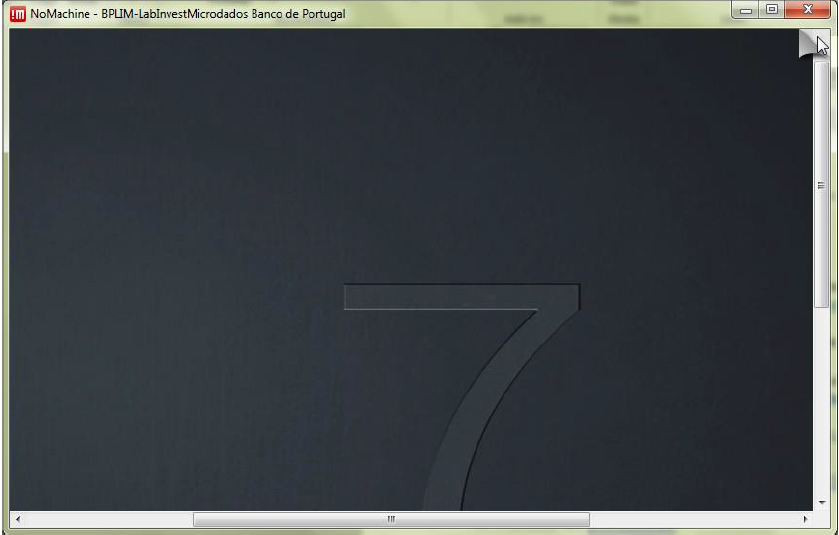
\includegraphics[width=4.72441in,height=3.01274in]{./media/image38.png}

\textbf{Step 5.13}: Click `Display'

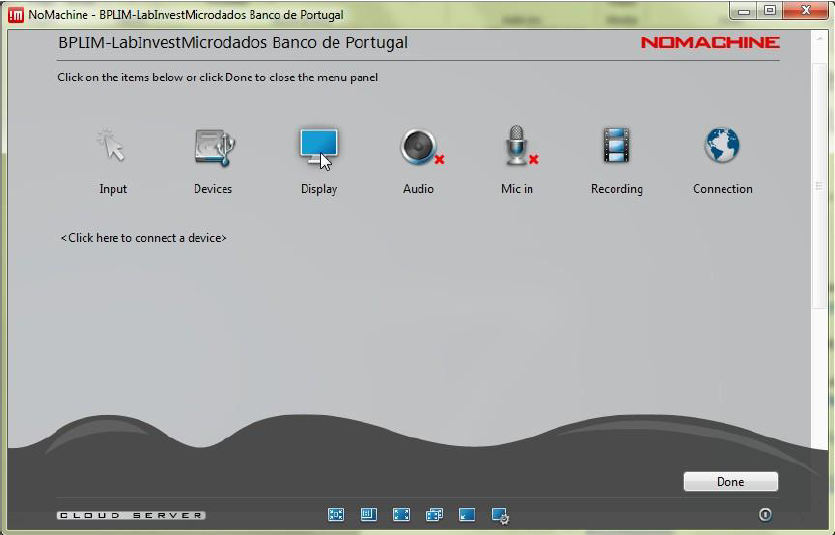
\includegraphics[width=4.72441in,height=3.0268in]{./media/image39.png}

\textbf{Step 5.14}: Click `Fit to window' and click `Done'

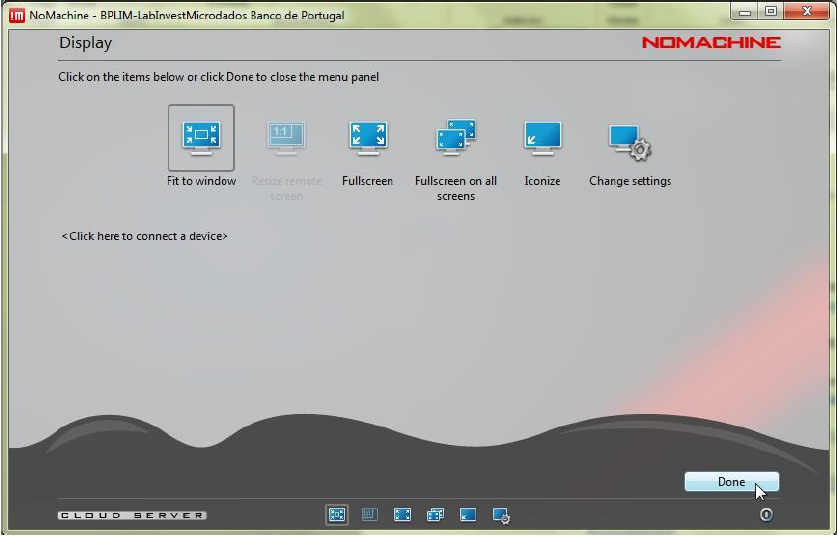
\includegraphics[width=4.72441in,height=3.02195in]{./media/image40.png}
\end{quote}

\hypertarget{appendix-5-browser-access}{%
\section{\texorpdfstring{{Appendix 5 -- Browser access}}{Appendix 5 -- Browser access}}\label{appendix-5-browser-access}}

\begin{quote}
Use a browser (recommended Chrome, Firefox, Opera or Safari) and go to
\url{https://bplim.bportugal.pt:4443}
\end{quote}

Configuring browser access

\begin{quote}
To a large extent the configuration of the access via browser is
similar to the configuration through the client NoMachine. However,
the features and performance are lower than the ``NoMachine client
access''.

In case you are using a Portuguese Keyboard, note that the keyboard
has to be set to Portuguese, as shown below, and even then some
characters may have to be specified on the virtual keyboard (depending
on the browser used). Please confirm the configuration of characters
on your keyboard.

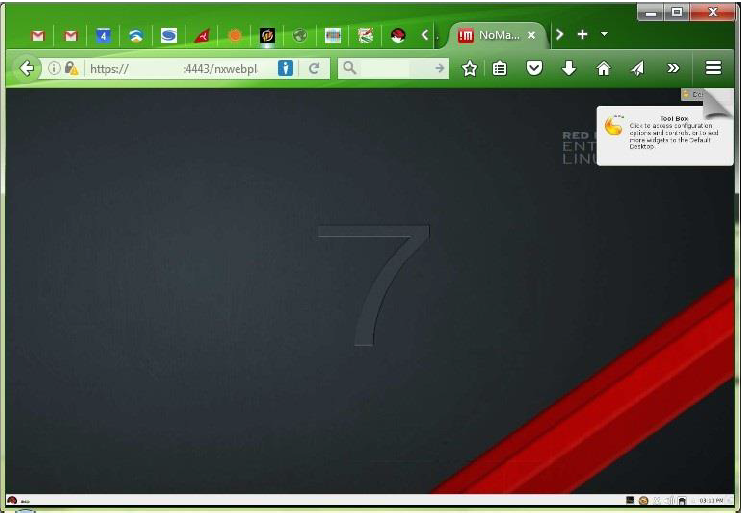
\includegraphics[width=4.72441in,height=3.26627in]{./media/image41.png}

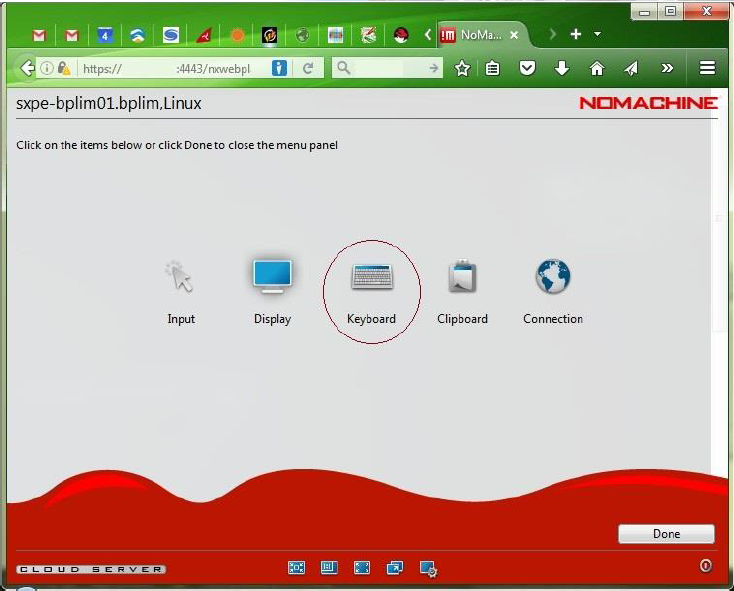
\includegraphics[width=4.72441in,height=3.80386in]{./media/image42.png}

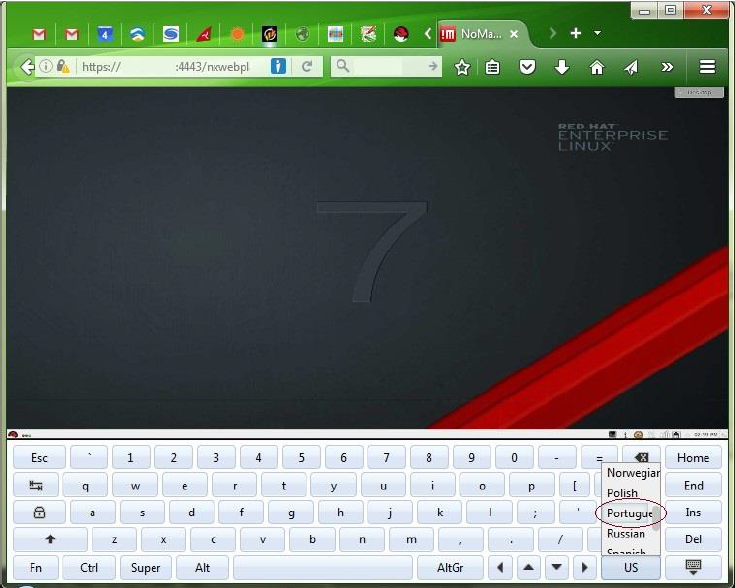
\includegraphics[width=4.72441in,height=3.77962in]{./media/image43.png}

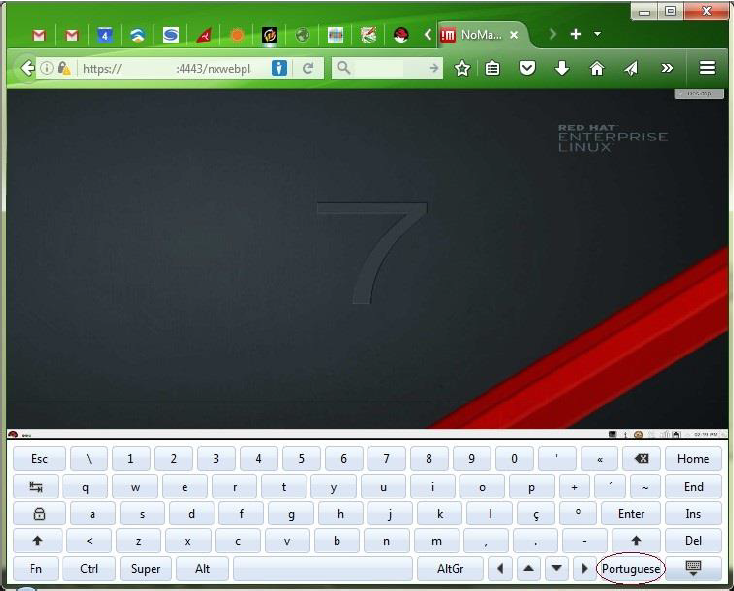
\includegraphics[width=4.72441in,height=3.80386in]{./media/image44.png}
\end{quote}

\hypertarget{appendix-6-frequently-asked-questions}{%
\section{\texorpdfstring{{Appendix 6 -- Frequently Asked Questions}}{Appendix 6 -- Frequently Asked Questions}}\label{appendix-6-frequently-asked-questions}}

\begin{enumerate}
\def\labelenumi{\arabic{enumi}.}
\tightlist
\item
  After the login in ``\url{https://webfa.bportugal.pt}'' I am not able to
  dowload NoMachine's setup file
\end{enumerate}

It may occur that a firewall is preventing the download. We have
verified such problem in some Universities and Governmental services.
Please try the download outside the firewall

\begin{enumerate}
\def\labelenumi{\arabic{enumi}.}
\setcounter{enumi}{1}
\tightlist
\item
  Mac users are not able to install NoMachine, receiving the following
  message
\end{enumerate}

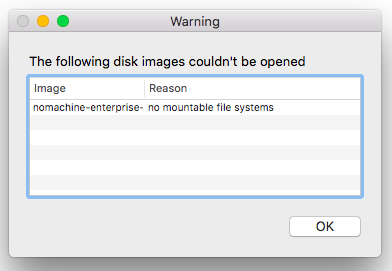
\includegraphics[width=2.16535in,height=1.49697in]{./media/image45.png}

Please check if your Mac OSX is updated. Temporary solution: download
NoMachine Enterprise Client from the official website, and run the
installation file:

\url{https://www.nomachine.com/download-enterprise/\#NoMachine-Enterprise-Client}

\begin{enumerate}
\def\labelenumi{\arabic{enumi}.}
\setcounter{enumi}{2}
\tightlist
\item
  NoMachine authentication failure
\end{enumerate}

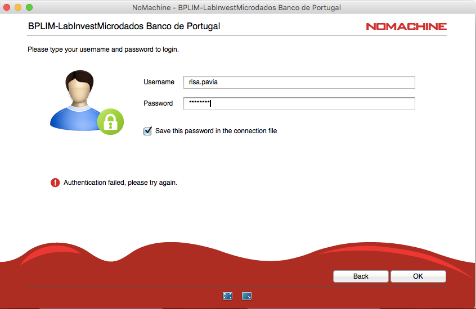
\includegraphics[width=2.16535in,height=1.40773in]{./media/image46.png}

\begin{itemize}
\item
  We have observed that some users who change their password within
  ``\url{https://webfa.bportugal.pt}'' later are not able to login within
  NoMachine (error message shown in the image above). In some cases it
  occurs due to a different keyboard layout. For example, if you have
  a Portuguese keyboard, but the website assumed a US keyboard, and
  your password contains a symbol like `ç', than you will get a ``wrong
  password'' message. Please check the keyboard layout that is active
  when you type the password. Alternatively, change the password after
  the first login with NoMachine. Use linux's command `passwd'.
\item
  Login fails and the system shows the message: "Could not connect to
  the server. Error is 138: Connection is timed out" Please check if
  your network has a strict firewall; e.g., some researchers are not
  able to reach BPLIM's server within their University network. Please
  check if in a different location, like at home, the connection
  works.
\end{itemize}

\begin{enumerate}
\def\labelenumi{\arabic{enumi}.}
\setcounter{enumi}{3}
\tightlist
\item
  User pressed `Lock' instead of `Log out' and the unlock/password
  does not work:
\end{enumerate}

\begin{itemize}
\item
  Check if the keyboard settings are correct (e.g., PT or UK)
\item
  Close the `NoMachine' connection and start a new one. Before the
  last step -before the 'Login'- right click and choose `Logout'.
  Double-click for the new connection
\end{itemize}

\begin{enumerate}
\def\labelenumi{\arabic{enumi}.}
\setcounter{enumi}{4}
\tightlist
\item
  ``Cannot see the screen in NoMachine'' (see image below)
\end{enumerate}

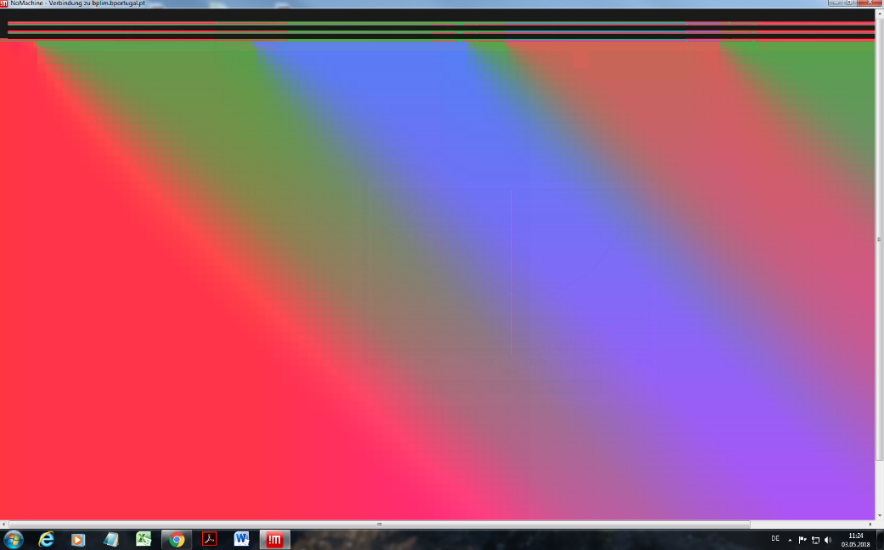
\includegraphics[width=4.01667in,height=2.49995in]{./media/image47.png}

\begin{enumerate}
\def\labelenumi{\arabic{enumi}.}
\setcounter{enumi}{4}
\tightlist
\item
  {OPTION A}: move your mouse on top the upper right
  corner of NoMachine, you should see a ``folded like sheet'',
  left-click your mouse, go to `Display', `Change settings', and click
  in `Disable client side hardware decoding'
\end{enumerate}


\includegraphics[width=1.56522in,height=0.15in]{./media/image48.png}

\begin{enumerate}
\def\labelenumi{\arabic{enumi}.}
\setcounter{enumi}{5}
\tightlist
\item
  {OPTION B}: Close the `NoMachine' connection and start a
  new one. Before the last step -before the 'Login'- right click and
  choose `Logout'. Double-click for the new connection
\end{enumerate}

\hypertarget{references}{%
\chapter{References}\label{references}}

\bibliography{book.bib,packages.bib}


\end{document}
